\documentclass[12pt]{article}

\usepackage{hcmus-report-template}

% Disable indentation on new paragraphs
\setlength{\parindent}{0pt}

% Line spacing 1.5
\renewcommand{\baselinestretch}{1.5}

% Optional: graphic path
% \graphicspath{PATH_TO_GRAPHIC_FOLDER}

% To use Times font family, uncomment this row
% \usepackage{mathptmx}

% To use roman section / subsection, uncomment these rows
% \renewcommand{\thesection}{\Roman{section}}
% \renewcommand{\thesubsection}{\thesection.\Roman{subsection}}

% Define course name, report name and report title.
\newcommand{\coursename}{CS163 - Data Structures}
\newcommand{\reportname}{Data Visualization}
\newcommand{\reporttitle}{Project Report}
\date{\today}

\newcommand{\studentname}{
\begin{tabular}{ll}
\end{tabular}
}

% Header
\lhead{\reporttitle}
\rhead{
HCMUS - Group 02\\
\coursename
}

% Footer

% ============ DOCUMENT ============
\begin{document}

\begin{titlepage}
\newcommand{\HRule}{\rule{\linewidth}{0.5mm}}
\centering

\textsc{\LARGE University of Science}\\[0.5cm]
\textsc{\Large VNU-HCM }\\[0.4cm]
\textsc{\large Faculty of Information Technology}\\[0.4cm]

\includegraphics[scale=.35]{img/hcmus-logo.png}\\[1cm] 

\huge{\bfseries{\reporttitle}}\\[0.5cm]
\large{\bfseries{Project: \reportname}}
\\[0.4cm]

\textbf{\large Course: \coursename}\\[0.5cm]
\textbf{\large Class: 24A02}\\[0.5cm]
\begin{minipage}[t]{0.4\textwidth}
\begin{flushleft} \large
\emph{Team members:}\\
\studentname
\end{flushleft}
\end{minipage}
{\large \today}\\[1cm]

\vfill
\end{titlepage}
	

\tableofcontents
\listoftables
\pagebreak

% \pagenumbering{arabic}
% \setcounter{page}{1}

\section{Introduction}


The project is part of our CS163 (Data Structure and Algorithm) course studied in HCMUS. It helps us to reinforce what we have learned in this course as well as has the first project to work and get used to OOP design - which we will learn later in CS202 (Programming System). The outcome of this project is to create a simple visualization application that can visualize some data structures and algorithms
\section{Group Information}
\subsection{Hoàng Đôn Thiện Hòa (23125035) - Leader}
\begin{itemize}
    \item  Management: Planning timeline, plans for the project.
    \item Coding Process:
    \begin{itemize}
        \item Work on the Graph logic part (ShortestPath, Kruskal, MST).
        \item Support work on Graph visualization.
        \item Support work on other parts.
        \item Fix bugs, control and optimize the code.
        \item Finalize and complete the project.

    \end{itemize}
    => Contribution Percentage: 23\%
\end{itemize}

\subsection{Nguyễn Lê Quốc Huy (24125100)}
\begin{itemize}
    \item Coding Process    
    \begin{itemize}
        \item Work on Graph Visualization.
        \item Participate in building program structure (design OOP).
        \item Work on coding and design common GUI 
        \item Code UI Controller.
        \item Work on LinearHashTable (logic part).
        \item Support work on AVL Tree (visualization and effect).
        \item Support work on program effect.
    \end{itemize}
    => Contribution Percentage: 27\%
\end{itemize}

\subsection{Lê Đức Thịnh (24125045)}
\begin{itemize}
    \item Coding Process    
    \begin{itemize}
        \item Work on logic for AVL Tree (Create, insert, move).
        \item Support work on LinearHashTable (visualization, functions: create, insert, remove, update).
        \item Highlight code for Linear Hash Table.
        \item Design the texture for buttons and relevant images (Dark/Light theme).
        \item Work on MenuTab for changing data structures.
    \end{itemize}
    => Contribution Percentage: 26\%
\end{itemize}

\subsection{Lê Văn Vĩ (24125050)}
\begin{itemize}
    \item Coding Process    
    \begin{itemize}
        \item + Working on logic and visualization for the Singly Linked List.
        \item Support working on the Command List.
    \end{itemize}
    => Contribution Percentage: 24\%
\end{itemize}
\section{Data Storage}
\subsection{Singly Linked List}
    We get a null pointer when the program is initialized called “head”, which is used for storing the first node of the singly linked list. Whenever we add a new element into the singly linked list, we allocate memory by using the “new” operator for the pointer next (member of the node). After all, the data is stored in dynamically allocated memory on the heap.
\subsection{Hash Table}
    In Hash table class, the data is simple saved in vector.
\subsection{Graph}
    The graph is constructed following adjacency list. 
    On adj list, we save all edge of this vertex into. 
    Moreover, on each edge, it links to 2 vertex pointer and have a total index to save to one total edge storage.
\subsection{AVL Tree}
    In AVL Tree form, there are 2 type of node: node for visual (called visual node) and node for logic work (called logic node).
\section{Project Architecture}
\subsection{Architecture}
    Contains 7 sub folders:
    \begin{itemize}
        \item .vscode: have many config file to run for Visual Studio Code.
        \item asset: contains images and sound file for prorgam.
        \item build: contains cmake build file and exe for Visual Studio Code.
        \item include: contains all include files of program.
        \item source: contains all cpp and main file.
    \end{itemize}
\subsection{Main structure of program}
    Firstly, program starts at main.cpp, declare application class and do application.run().
    This application object when constructing inits main window, connect with audio device and construct many other variables.
    The program is offically starting with run() function. This function contains main while loop with many case (condition) to open current chosen form: FormStart, Menu, About us or AVL, Linear HashTable, Singly Linked List and Graph.
    At the beginning, first form will be FormStart, which has some button to go to Menu, About us, Custom setting or exit program.
    With each form, there are 3 main functions (except constructor and destructor): 
    \begin{itemize}
        \item  int run(): contains while loop, return next form will go to.
        \item void handle(): catch event and control behavour of controller on real time;
        \item void draw(): only for drawing UI;
    \end{itemize}
    For data structure form, using OOP inherit, we observe that there are many same function between many data structure function. So, all data structure form will be inherited from one exactly Form class with 3 main functions like above and some feature virtual functions to add, remove, update,... (for Derived class to override in the future);
    

\section{Implementation Details}
\subsection{Include Files}
\begin{itemize}
    \item UI Controller: 
TextureButton.h,
Controller.h,
Console.h,
Button.h,
ColorPointer.h,
TextureButton.h,
Controller.h,
Console.h,
Button.h,
ColorPointer.h,
DijkstraMargin.h,
Bubble.h,
Label.h,
SunMode.h,
AVLNode.h,
Vertex.h,
ValueScroll.h,
ImageTab.h,
ProgressBar.h,
MenuTab.h,
EmptyButton.h,
TextBox.h,
FileDropBox.h,
LabelExtra.h,
HeapVisual.h,
ColorBox.h,
Edge.h,
DSU.h,
GIF.h,
MinHeap.h,
TextButton.h,
TabBox.h,
DynamicColorCircle.h,
    \item Container UI: 
MenuBox.h,
Container.h,
    \item Combine Control: 
MoveLabel.h,
MoveButton.h,
MoveTexture.h,
MoveContainer.h,
    \item Logic control: 
Clock.h,
CommandLists.h,
    \item Form: 
AboutUsForm.h
Graph.h,
AVLTree.h,
LinearHashTable.h,
SinglyLinkedList.h,
Application.h,
FormStart.h,
Form.h,
Menu.h.
    \item Effect: 
ZoomInTransition.h,
SlowMotion.h,
VerticalOpen.h,
Move.h.
    \item General: 
GUI.h,
RaylibExtra.h,
IncludePath.h,
Global.h,
SettingPackage.h,
General.h.
[see more in Appendix]
\end{itemize}
\subsection{Common flow}
Although, there are so many class, all of them both have 2 main functions: 
\begin{itemize}
    \item handle(): Be called on every loop, to catch event and adjust variable itself;
    \item draw(): Only used to draw this UI (some logic controller will have an empty draw())
\end{itemize}
Furthermore, most of UI controller are inherited from class Controller, so they both have functions: setPosition(...), getPosition(), setSize(...), getSize(), ...;

\subsection{Step by step flow}
The step by step is controlled by class CommandList.
It's simple that we add a code represent for some work of visuallization to queue. To go next, we get front of queue, pop it and push it to reverse queue. To turn back, we get front of reverse queue, pop it and push it again to queue.
To combine CommandList to main form, the form will be inherited CommandList and override FetchNextCommand() and FetchPrevCommand().
Moreover, we call CommandList handle() from Form.handle() to ensure FetchNext functions is called after a specified time.
\subsection{About custom feature}
To easy to change many attribute in same time, we firstly declare a new class contains 1 type of Controller, divide to ButtonSetting and TextSetting, and a class include both of them - FormSetting.
So, in setting form, when change any attribute or light/dark theme, we will change a pointer of FormSetting and pass it address/pointer to other form.
Note that: we use a pointer in many form to transfer the data to many sub-controller in form.
\subsection{Some common UI effect}
In most of UI effect controllers, we declare 2 types of functions: set and get.
Like Move effect, there are setPosition and getPosition function. So, to use them, we will combine it with other UI controller, inherit them, overriding set and get function and call it from derived class handle.
A few remain effect of function, it is easier to control, like zoom in. It contains only 1 main function: handle (except some other function to start or get some attribute or progress).
It is simple that this effect class will have a pointer of Controller to link to other UI, and use the properties of OOP, with some virtual functions from base class like setPosition/ getPosition and control linked class through these function.
\section{Technical Problems}
\begin{itemize}

    \item There were several problems we faced which need to be tackled during the project: 
    Main Program Structure: Initially, we found it challenging to build the main program due to its many separate yet interrelated components. After a discussion, we decided to adopt an Object-Oriented Programming (OOP) approach, organizing the program into distinct objects. This decision significantly improved project manageability and enhanced work efficiency.
    \item When first approaching the GUI, understanding how the program works can be quite challenging - especially the handling and drawing processes, which often feel unfamiliar to beginners. We spent a significant amount of time reading books and searching online resources. Eventually, we gained enough knowledge to start building the program.
    \item When Creating the Animation and Progress Bar: Creating animations for the program was the most challenging part. We encountered countless bugs during the animation development. Similar difficulties arose when implementing the progress bar (both stepping forward and backward). By diving deeper into the properties of the data structures and applying OOP design principles, and with a lot of enthusiasm, we supported each other and managed to overcome all the obstacles.

\end{itemize}




\section{Feature Demonstration}
\subsection{demo by capture}
\begin{center}
    Light theme 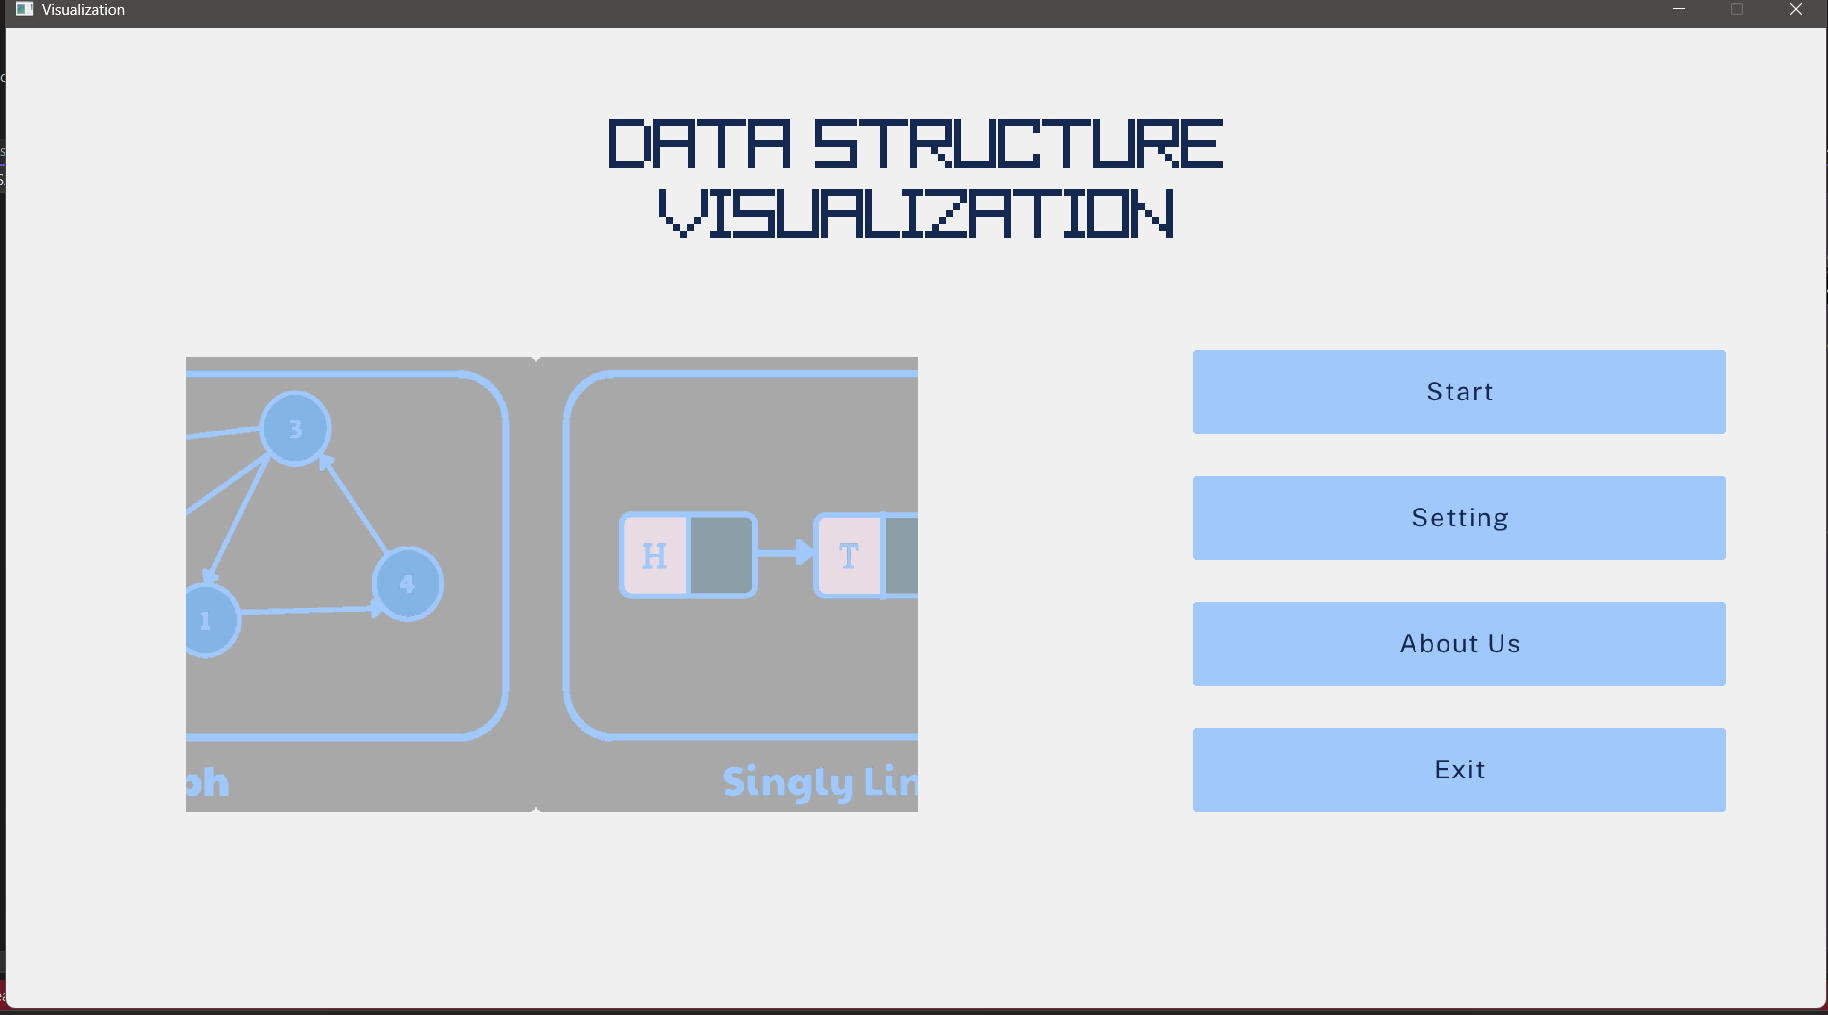
\includegraphics[scale=.35]{img/start_light.png} 
    
    Dark theme 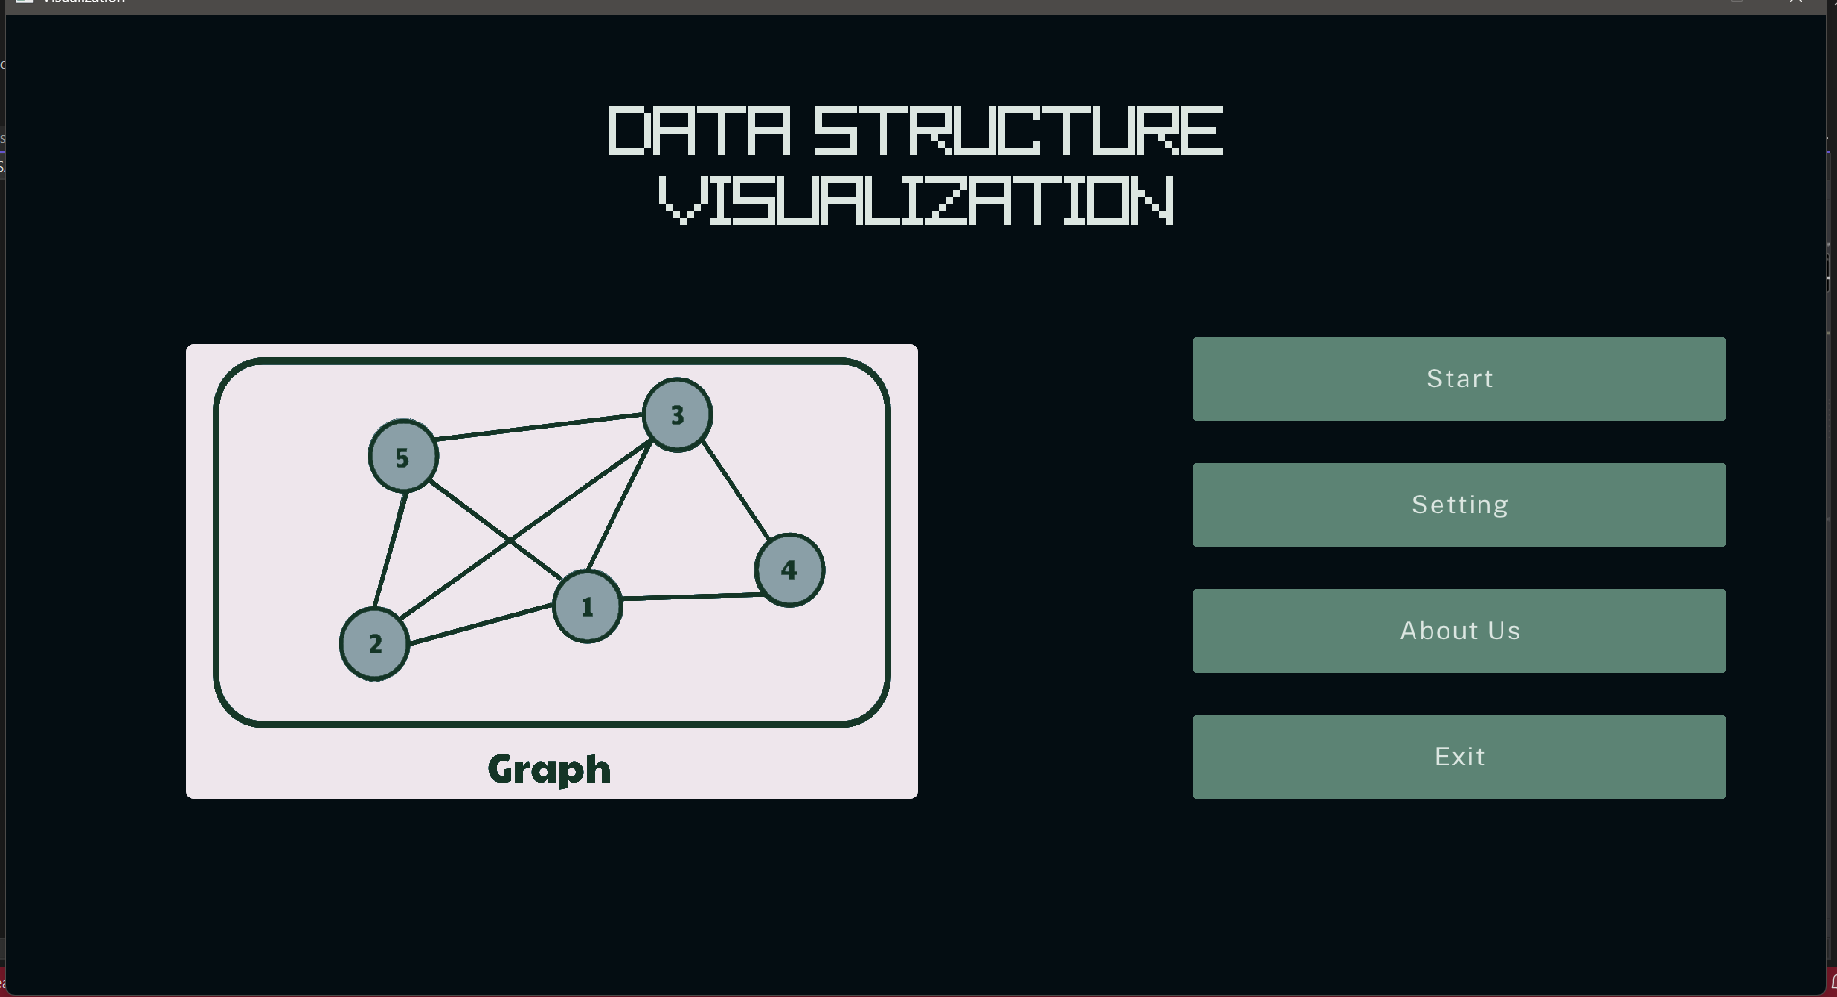
\includegraphics[scale=.35]{img/start_dark.png}  
    
    Setting 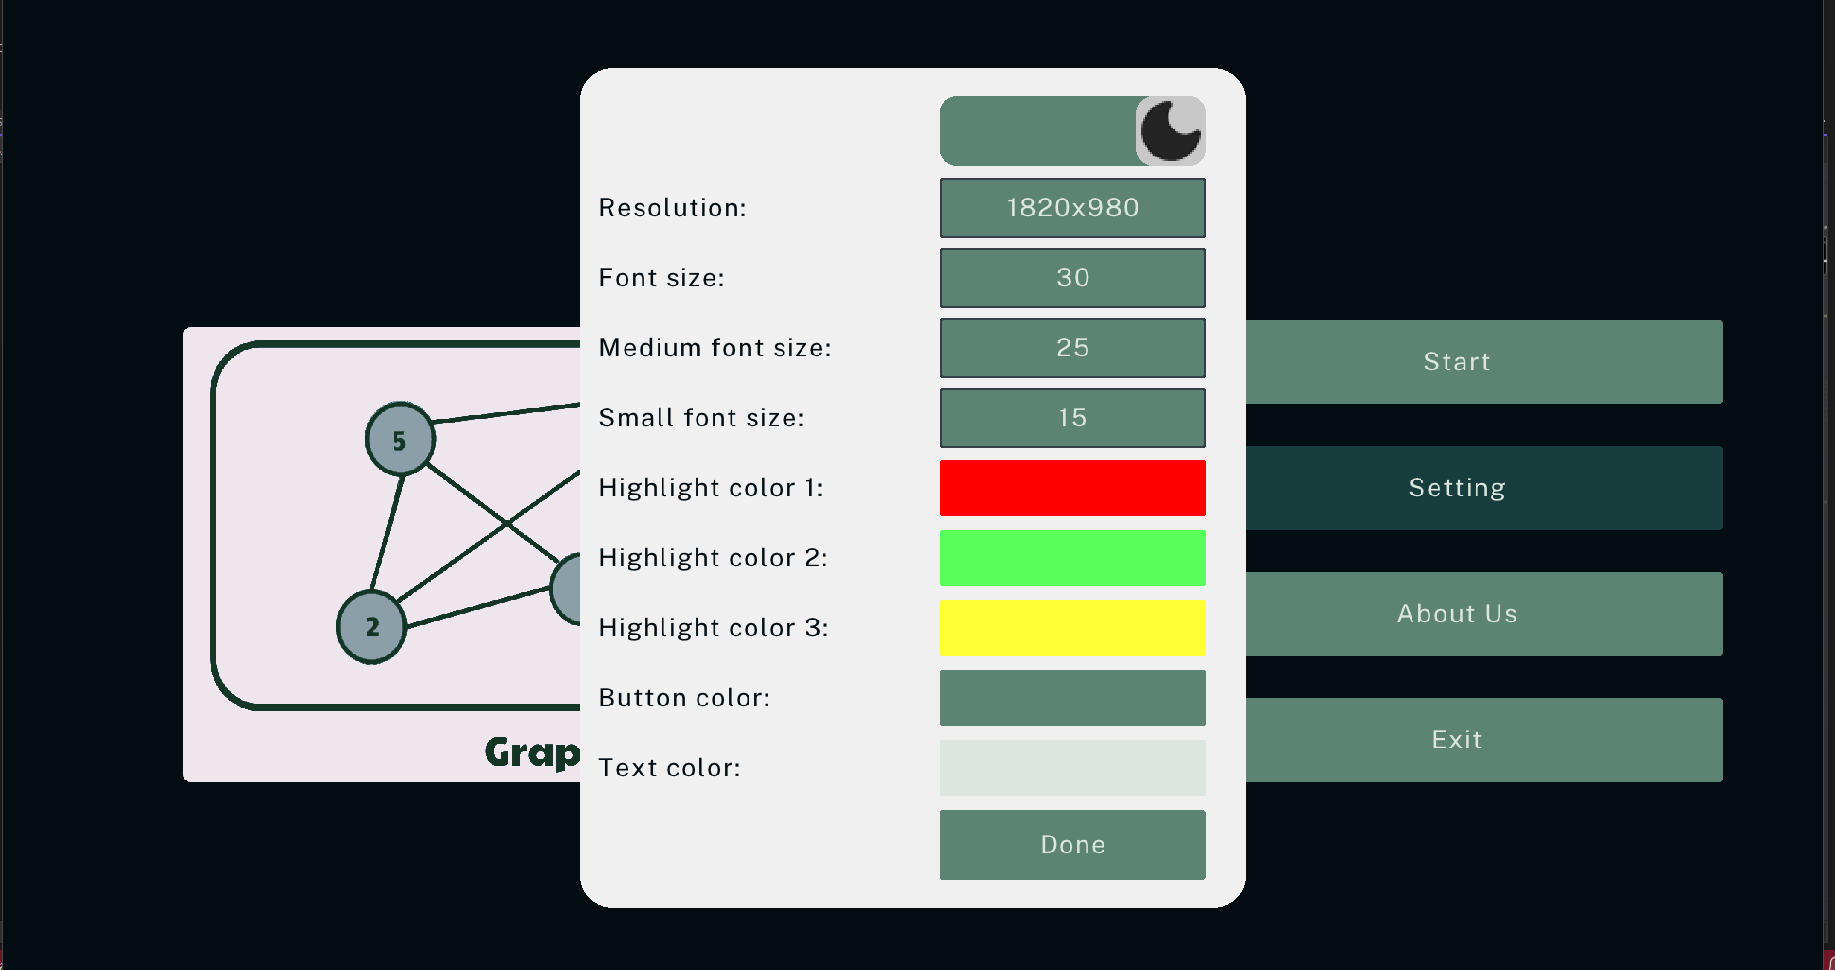
\includegraphics[scale=.35]{img/setting.png}
    
    About Us     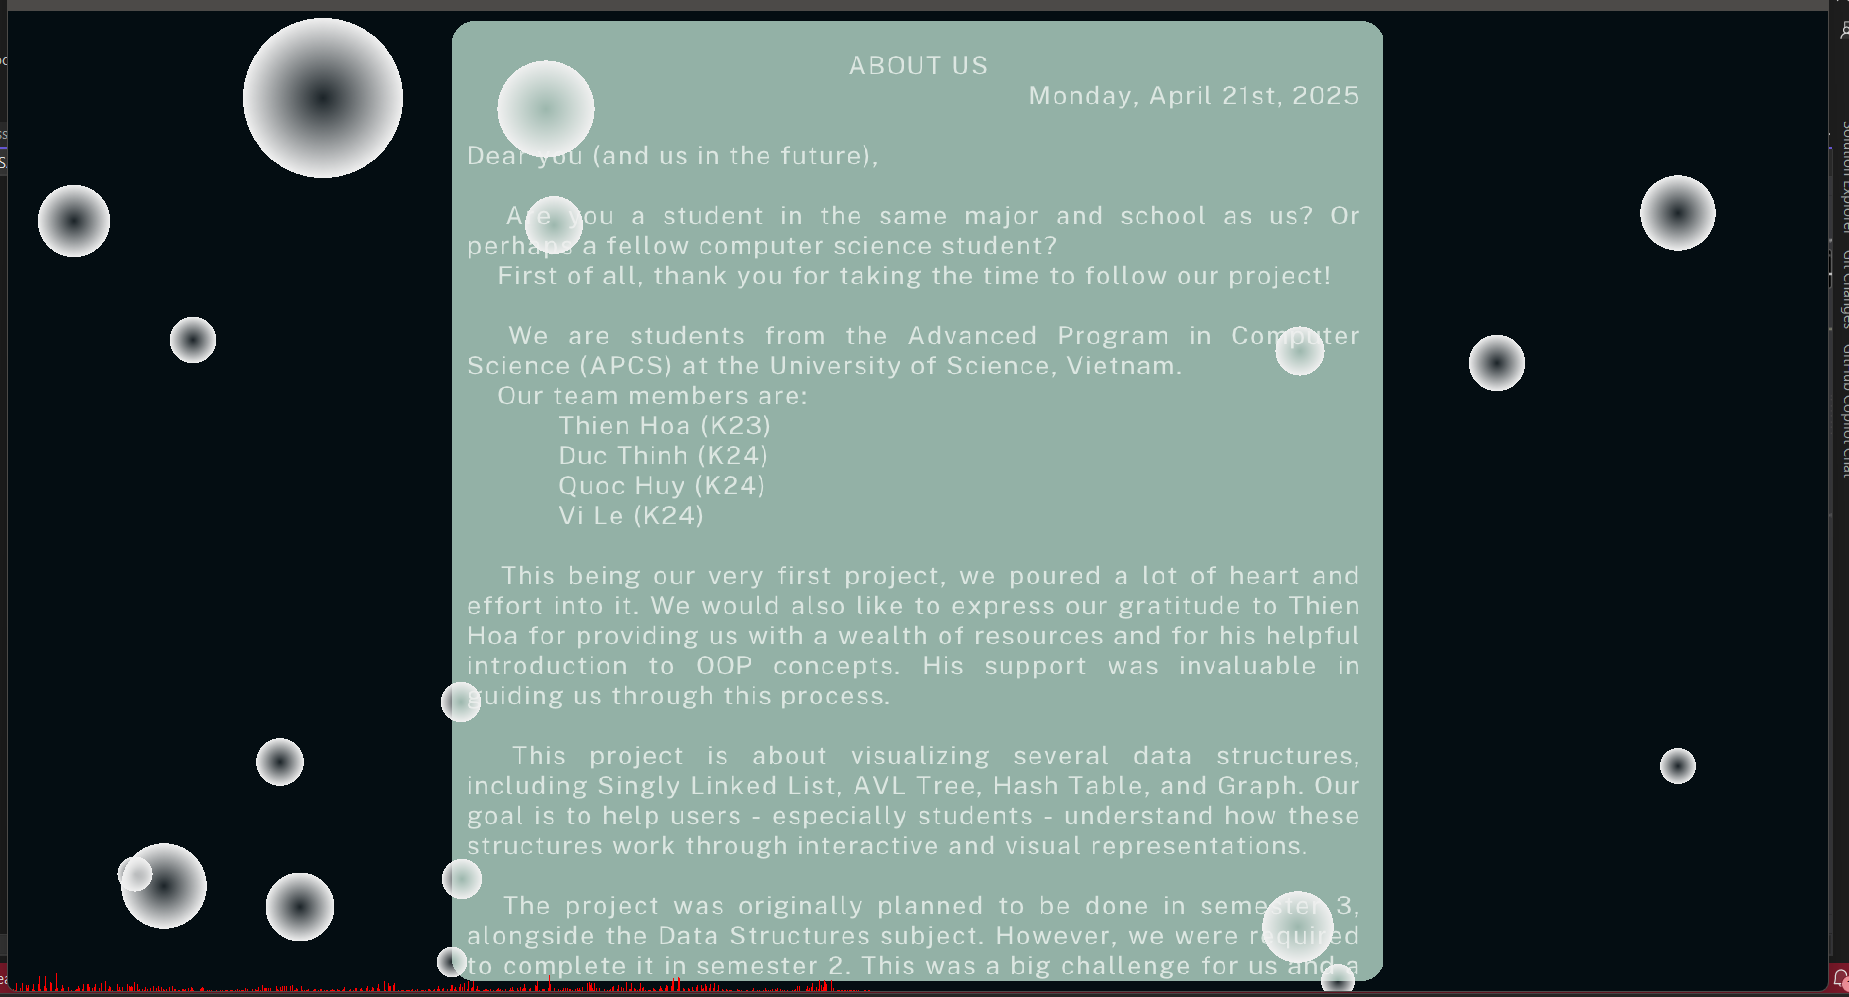
\includegraphics[scale=.35]{img/aboutus.png} 
    
    Menu 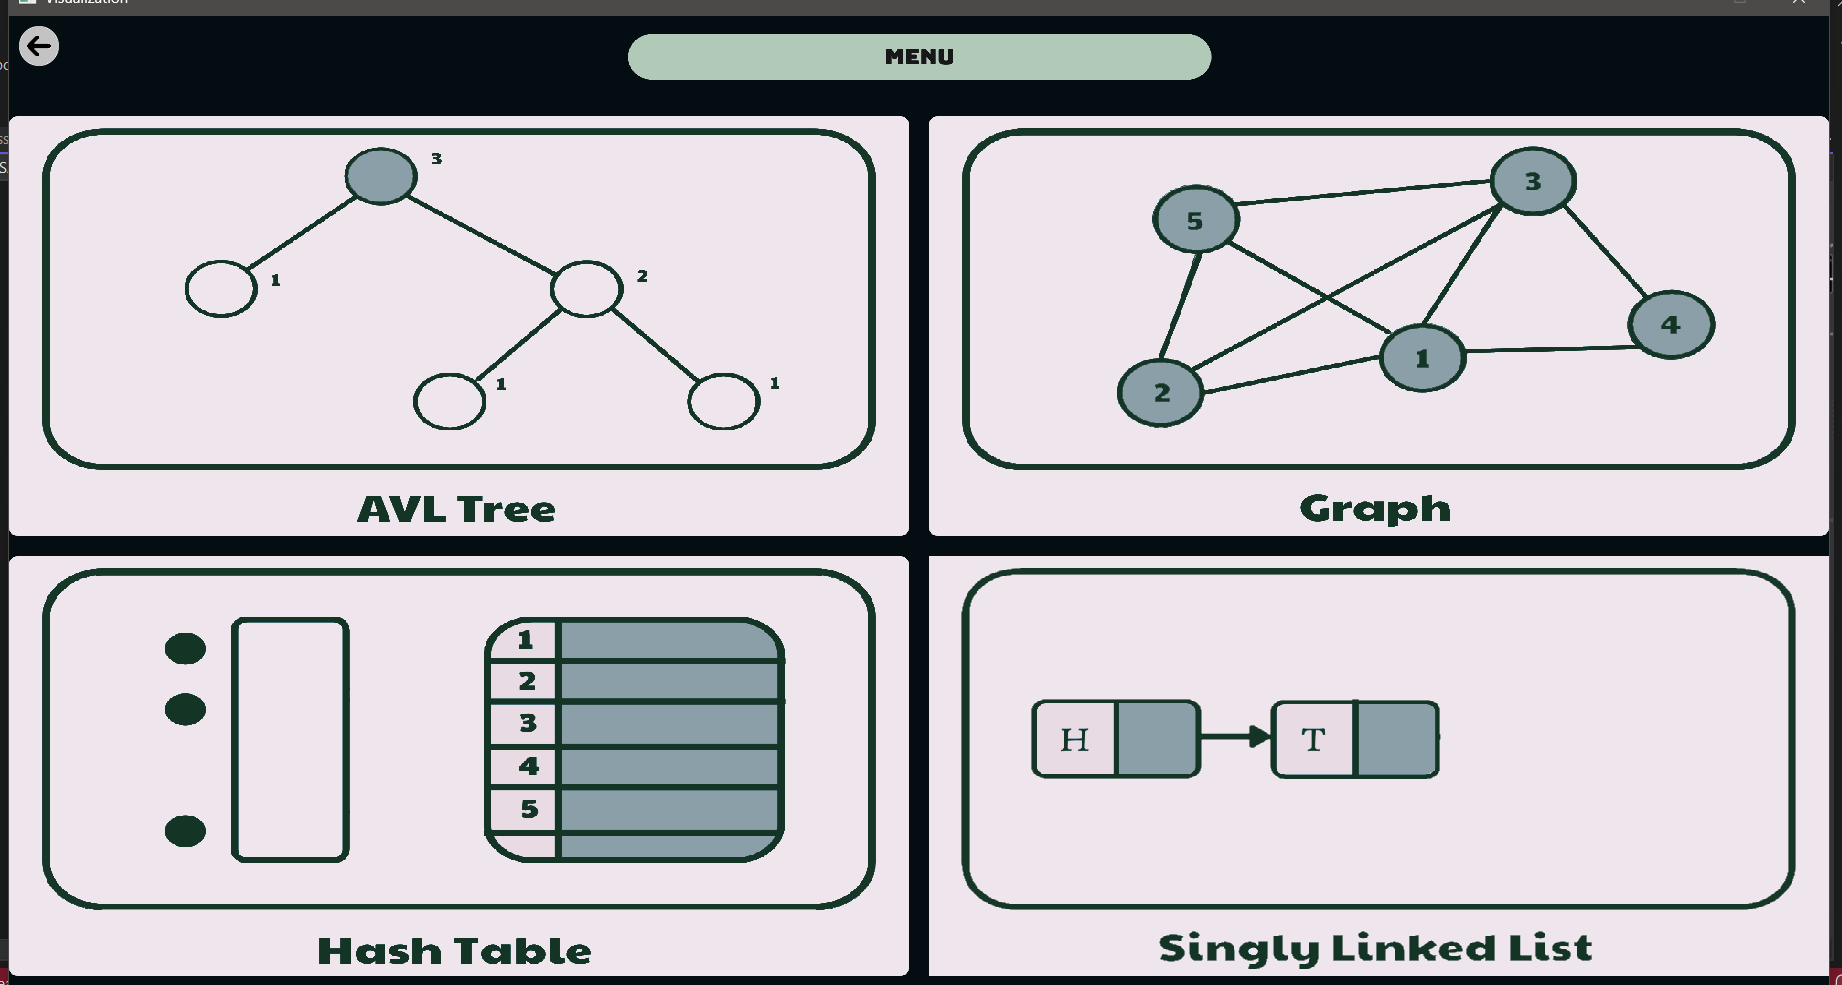
\includegraphics[scale=.35]{img/menu.png}
    
    AVL Tree 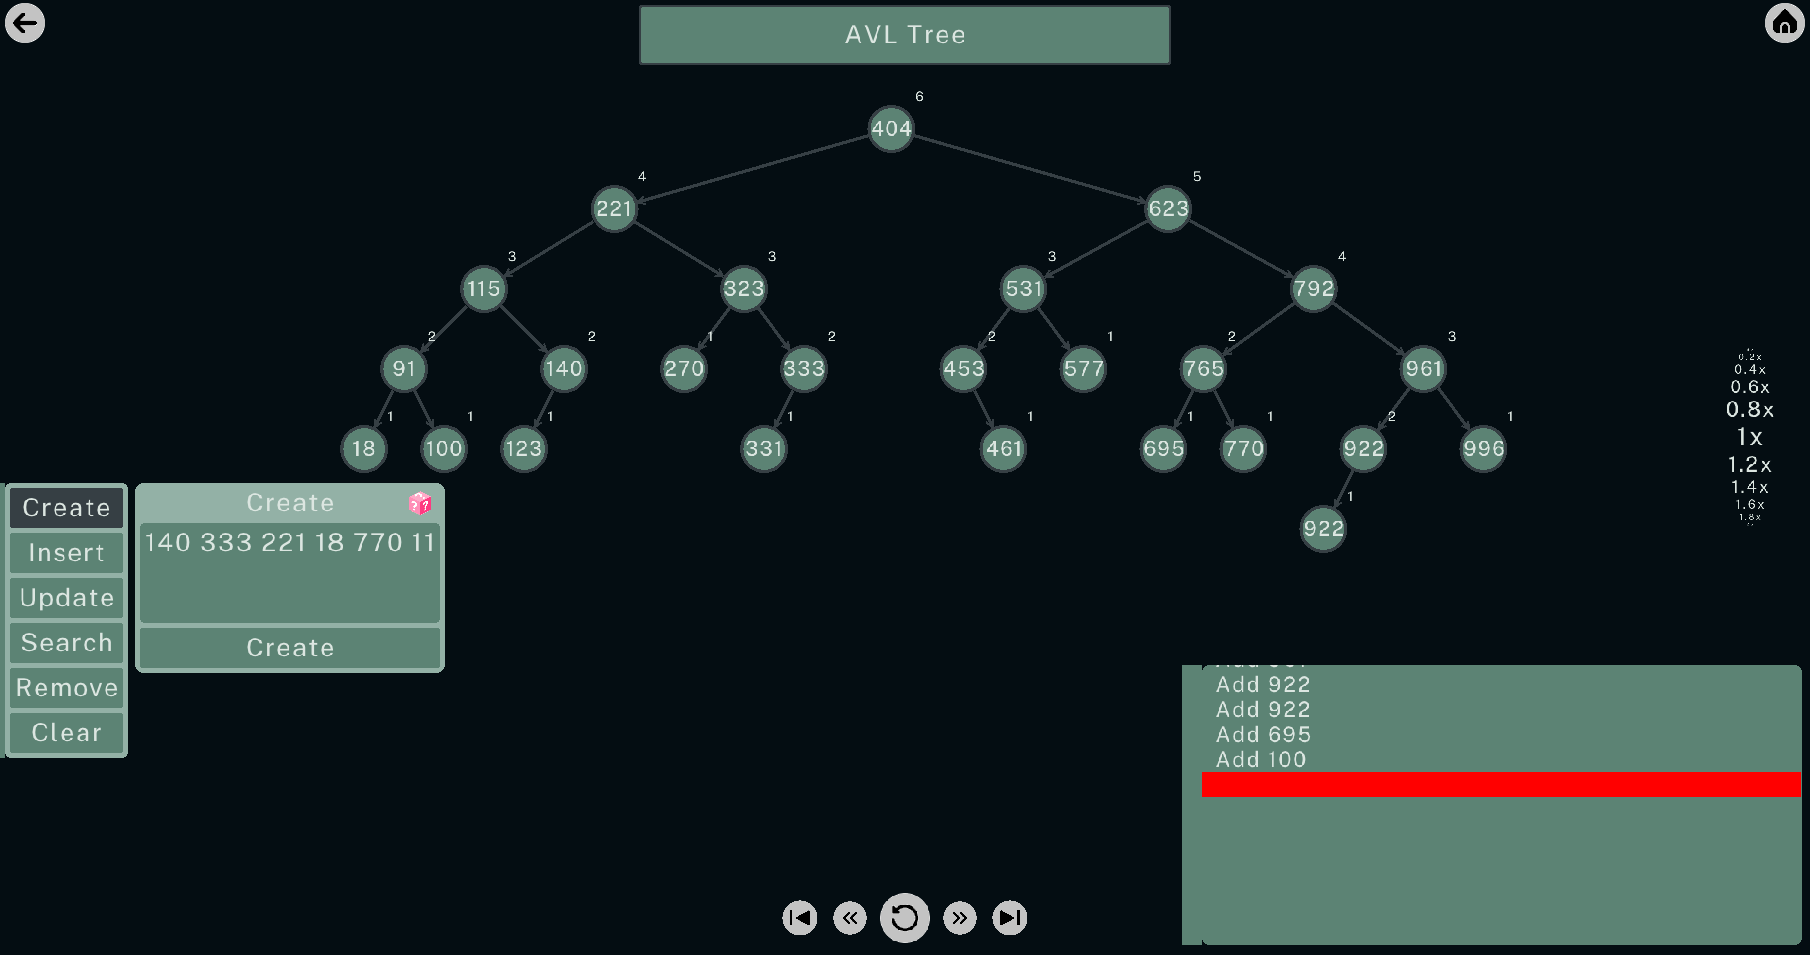
\includegraphics[scale=.35]{img/avl.png} 
    
    Hash table 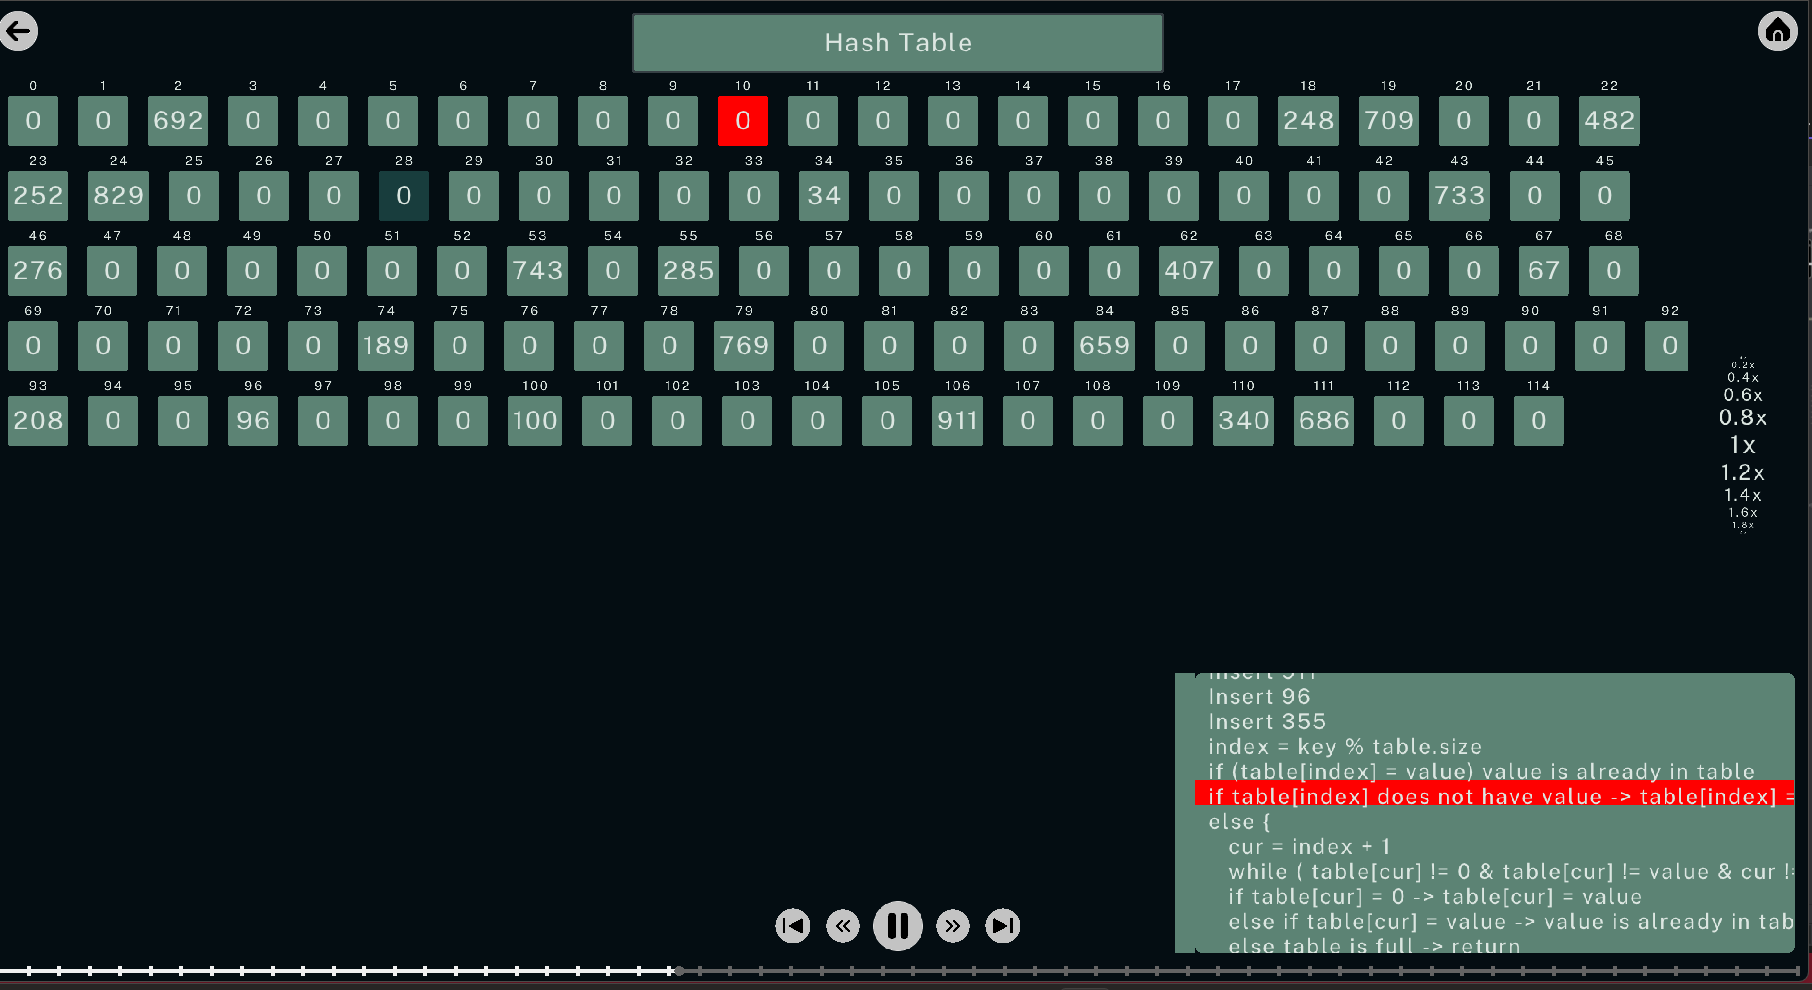
\includegraphics[scale=.35]{img/hashtable.png}
    
    Graph 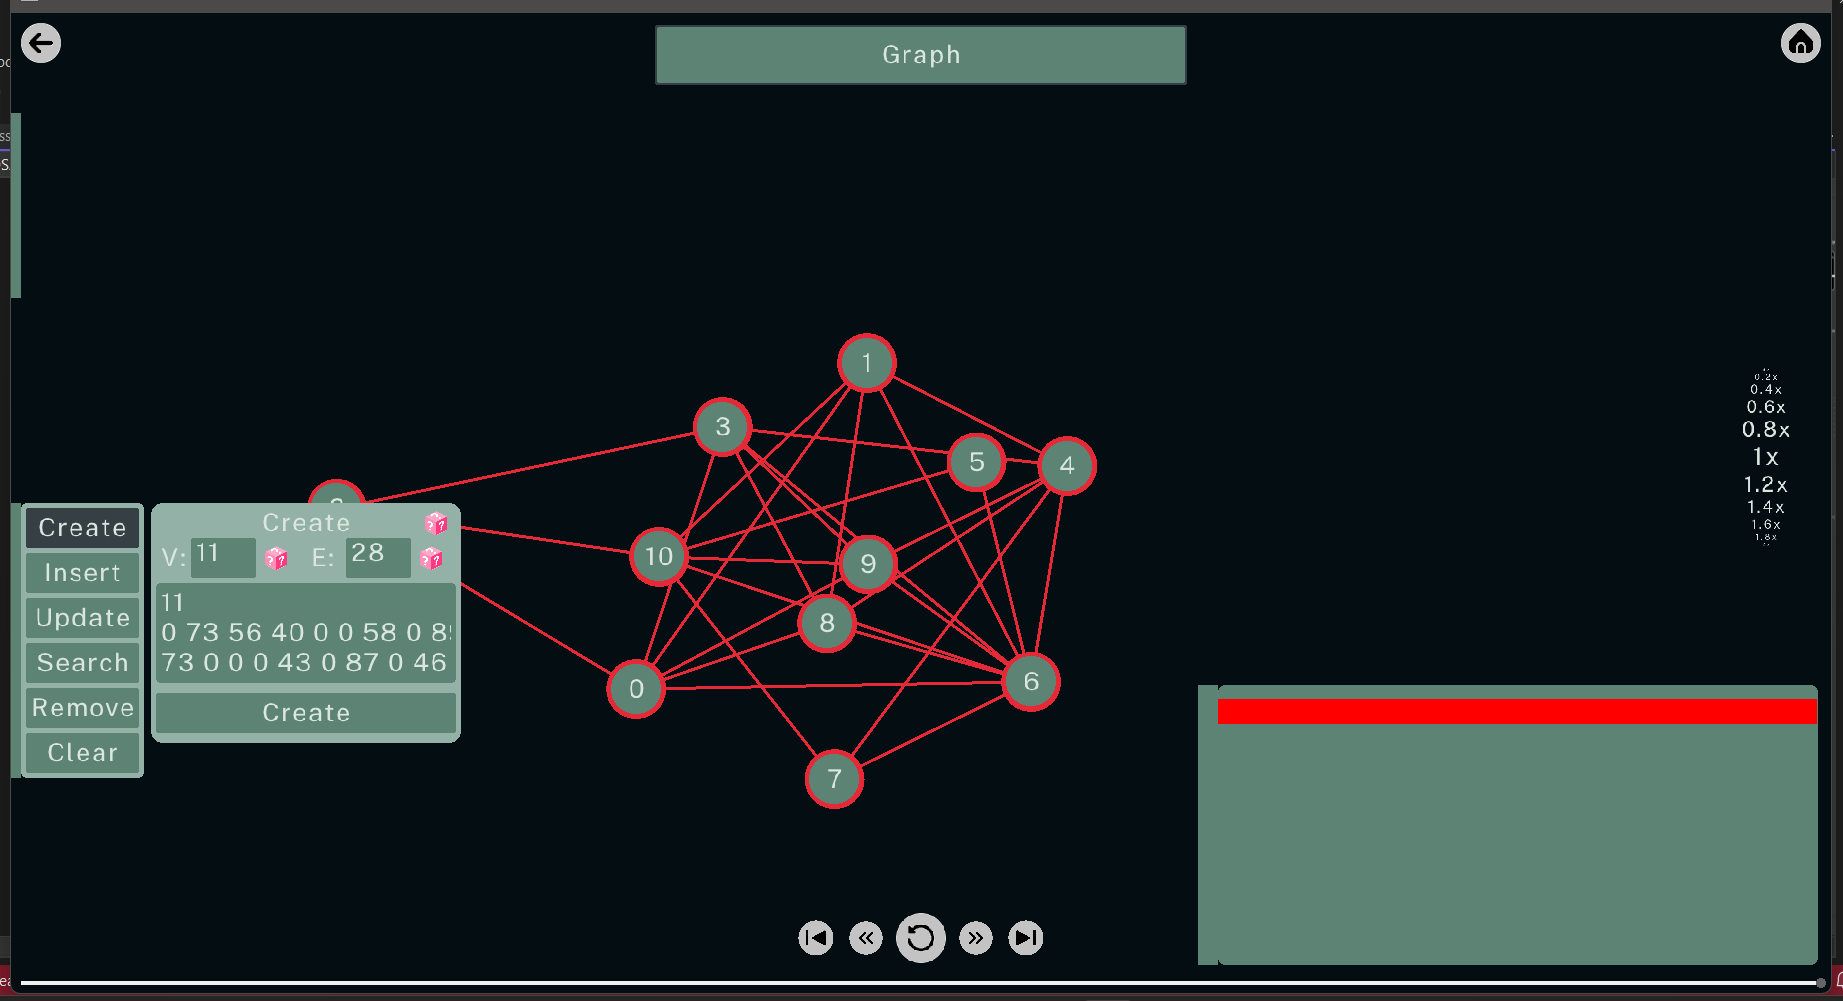
\includegraphics[scale=.35]{img/graph.png} 
    
    Algorithm in graph 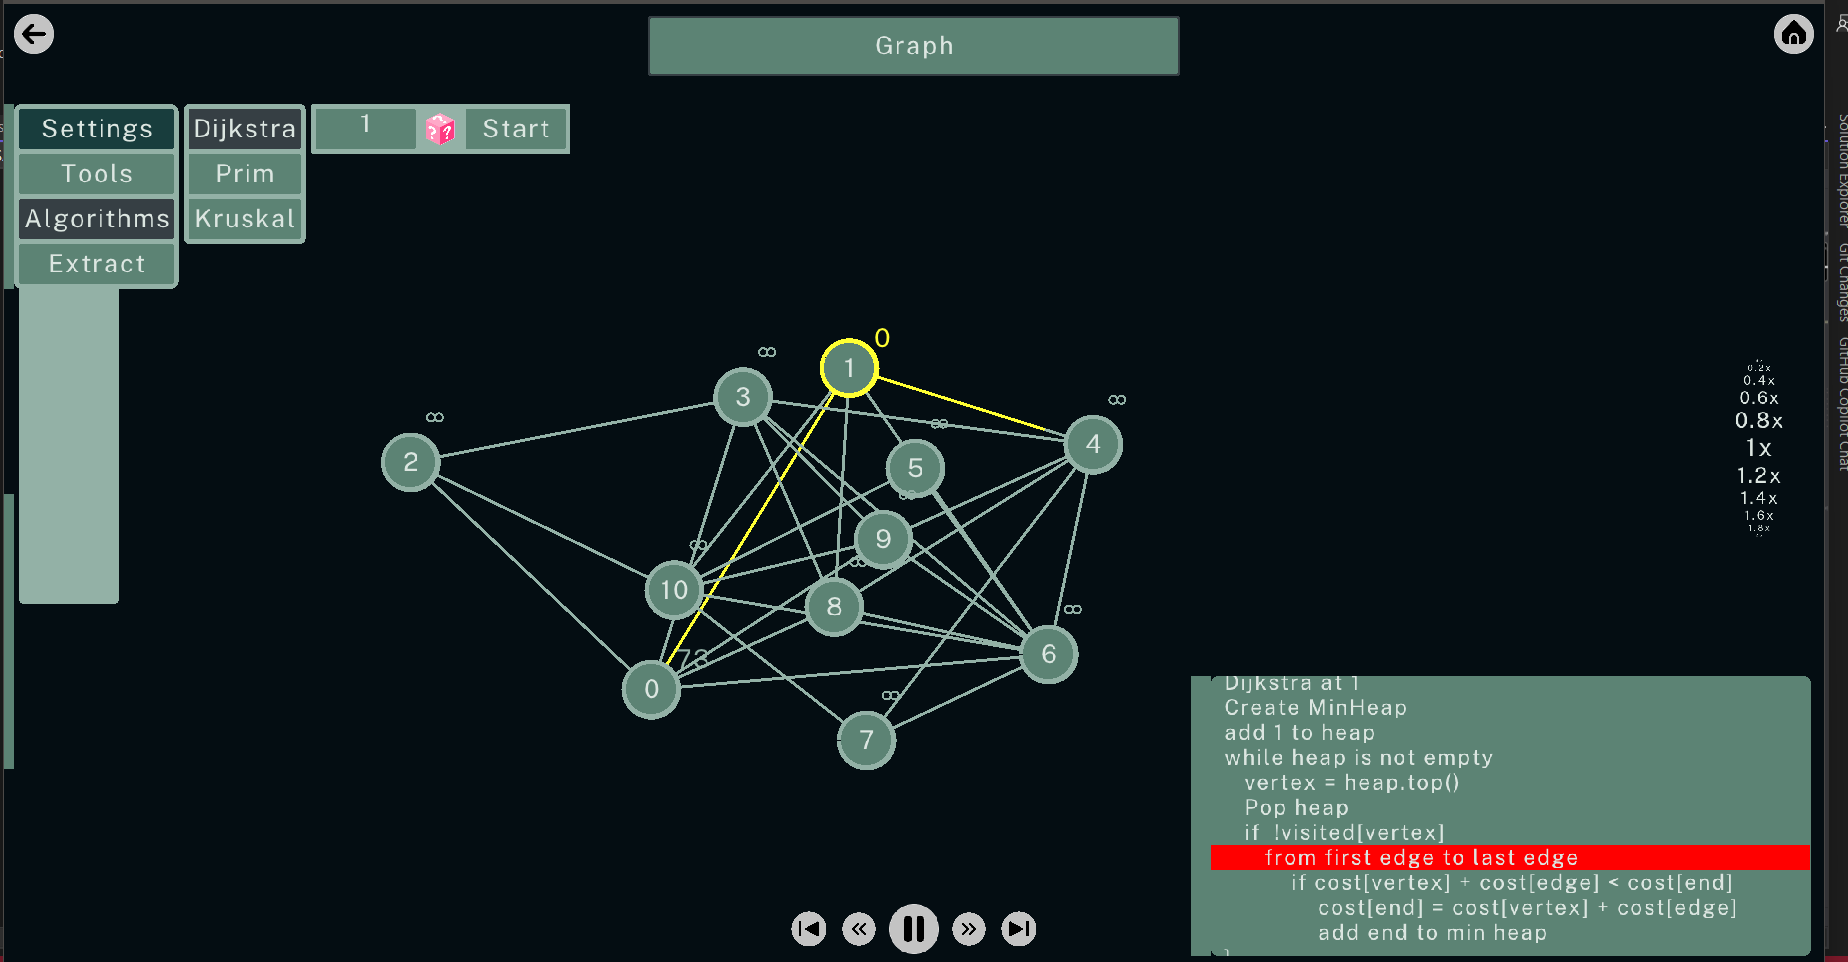
\includegraphics[scale=.35]{img/algorithm.png} 
    
    Singly linked list 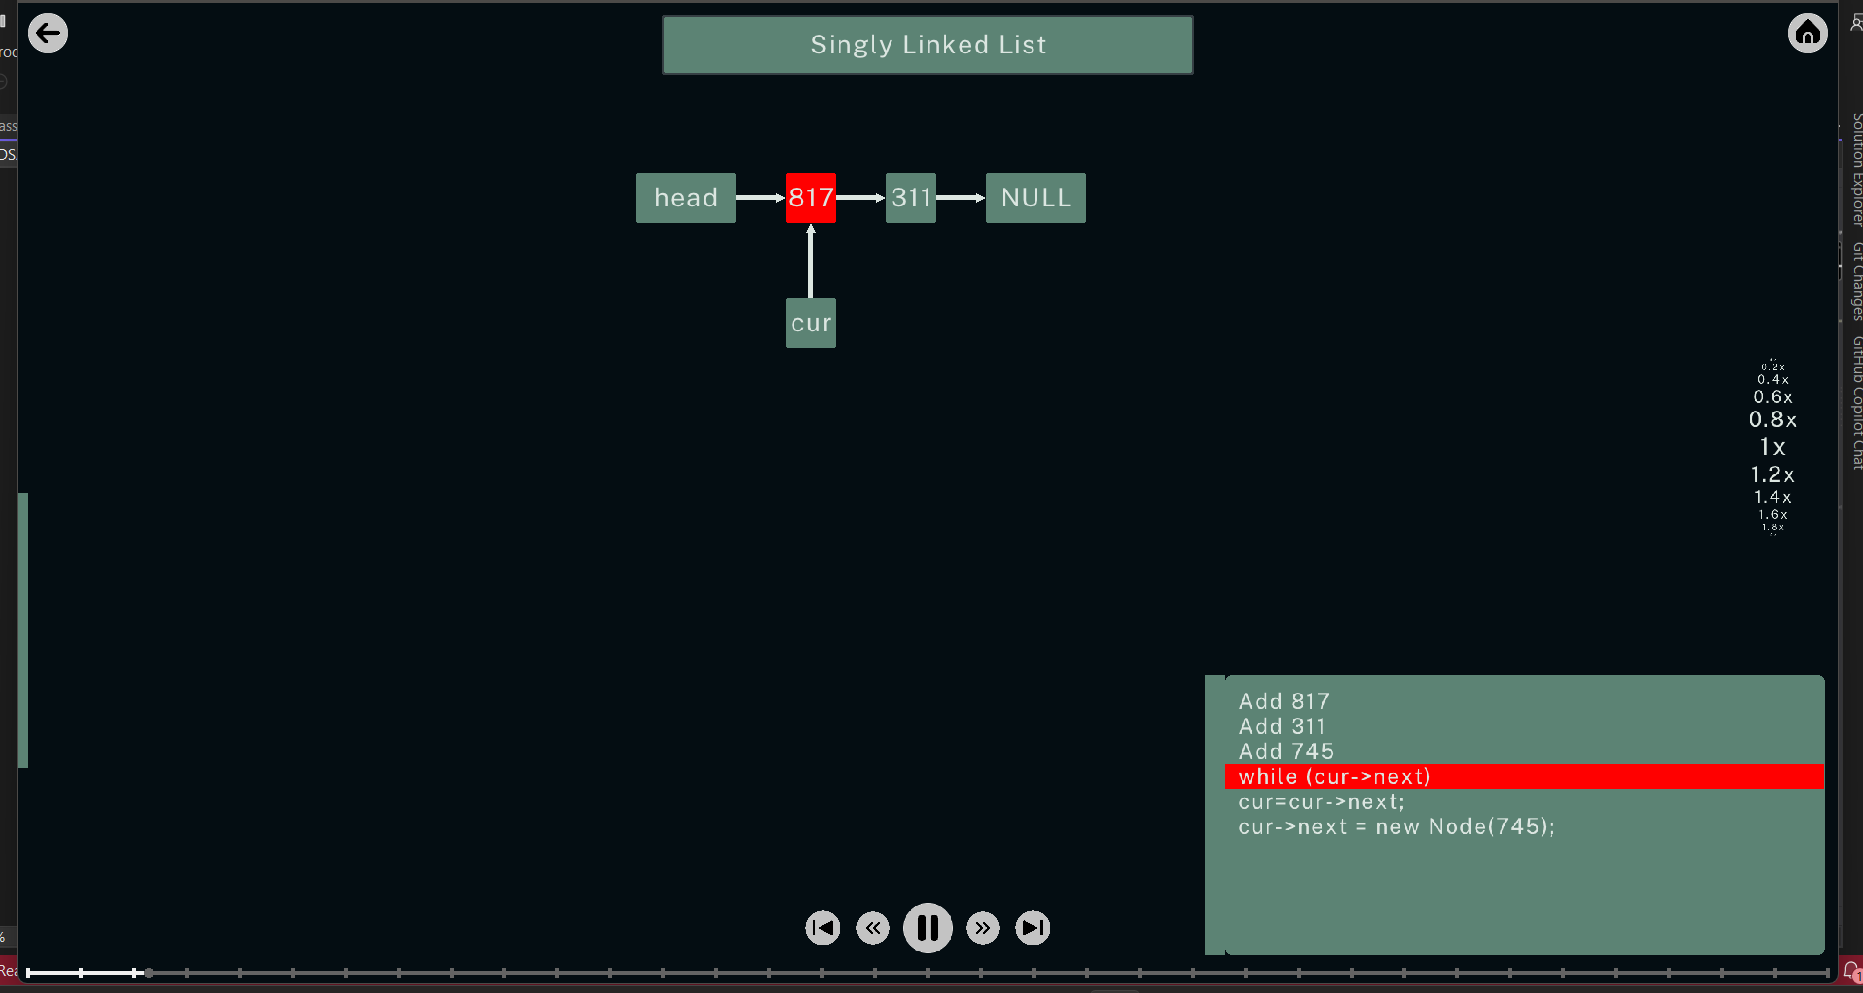
\includegraphics[scale=.35]{img/sll.png} 
\end{center}

\section{Conclusion}
Our project can demonstrate Linked List, Hash Table, AVLTree and Graph (Dijkstra, Prim, Kruskal) … In future, we may develop other structures and algorithms.

\section{Appendix}
\subsection{DijkstraMargin}
\begin{lstlisting}[language=C++]


class Dijkstra_Margin {
public:
    float           getValue() const;
    virtual void    setValue(const float& value),
                    draw();
private:
    float           m_value;
};






\end{lstlisting}

\subsection{Bubble}
\begin{lstlisting}[language=C++]


class Bubble: public Controller {
public:
    Bubble();
    float               getRadius() const;
    virtual void        handle() override,
                        draw()   override;
    
    virtual void        setRadius(const float& radius),
                        setColor(const Color& color);
    ~Bubble();
private:
    float               m_radius;
    Color               m_color_a, m_color_b;
};






\end{lstlisting}

\subsection{AboutUsForm}
\begin{lstlisting}[language=C++]


class AboutUsForm {
public:
    AboutUsForm(FormSetting form_setting, const Vector2& window_size);
    int             run();
    virtual void    handle(),
                    draw();
    ~AboutUsForm();
private:
    float           *music_sample, 
                    music_length, music_current,
                    bubble_velocity;
    Wave            wave;
    vector<float>   music_show;
    size_t          samples_size, current_index;
    Music           music;
    Vector2         m_window_size;
    FormSetting     form_setting;
    MoveContainer   main_container;
    LabelEx         main_letter;
    vector<Controller*> children;
    vector<Bubble>      bubbles;
    Clock               clock;
};




\end{lstlisting}

\subsection{MoveLabel}
\begin{lstlisting}[language=C++]


class MoveLabel: public Label, public Move {
public:
    virtual void    setPosition(const float& x, const float& y),
                    handle();
    Vector2         getPosition() const;
};






\end{lstlisting}

\subsection{TextureButton}
\begin{lstlisting}[language=C++]


class TextureButton : public Button {
public:
    TextureButton();
    int             getStage() const;
    virtual void    handle()                                            override,
                    draw()                                              override,
                    setSize(const float& width, const float& height)    override,
                    setButtonStage(const int& index, const string& source, const string& hover_source),
                    Hover();

    void            next(), back(), go(const int& index);
    ~TextureButton();
protected:
    int               source_pointer,
                      hover_remain_time;
    vector<Texture2D> m_sources;
    vector<Texture2D> m_sources_hover;
};





\end{lstlisting}

\subsection{Controller}
\begin{lstlisting}[language=C++]


class Controller {
public:
    Controller();
    virtual bool    isHovered() const,
                    isFocus() const;
    virtual void    handle()    ,
                    draw()      ,
                    setPosition(const float& x, const float& y),
                    setSize(const float& width, const float& height);
    virtual Vector2 getSize() const,
                    getPosition() const;
    virtual void    update();
    ~Controller();
protected:
    Vector2         m_position,
                    m_size;
};






\end{lstlisting}

\subsection{Console}
\begin{lstlisting}[language=C++]


class Console : public TextButton, public Move {
public:
    Console(ButtonSetting *b_setting, TextSetting* t_setting);
    int             getFillLine() const;
    virtual void    InsertNextSubCommand(const std::string& log),
                    InsertNextMainCommand(const std::string& log),
                    PushBackMainCommand(const std::string& log),
                    PushBackSubCommand(const std::string& log),
                    GotoCommandLine(const float& progress),
                    goUp(),
                    goDown(),
                    clear(),
                    handle()                                    override,
                    draw()                                      override,
                    setSize(const float& width, const float& y) override,
                    setText(const std::string& str)             override,
                    setTextOrigin(const Vector2& origin),
                    setEnable(const bool& enable),
                    setPosition(const float &x, const float &y) override;
    Vector2         getPosition() const override;
    bool            isEmpty();
    ~Console();
private:
    bool            m_is_enable;
    float           min_x = 0,
                    min_y = 0,
                    max_width = 0,
                    max_height = 0,
                    current_line = 0;
    int             line_cursor = 0,
                    main_line_cursor = 0,
                    current_add = 0;
    void            BeforeGoUp(),
                    BeforeGoDown(),
                    update_tail();
    std::vector<std::string>    m_list;
    std::vector<bool>           temporary;
    Vector2     m_origin = { 0, 0 },
                m_delta = { 0 , 0 },
                m_fixed = { 0, 0 };
    Clock       clock;
};






\end{lstlisting}

\subsection{Button}
\begin{lstlisting}[language=C++]


class Button: public Controller {
public:
    Button();
    bool                isHovered() const override,
                        isPressed() const;
    virtual void        handle()        override,
                        draw()          override;
    ~Button();
protected:
    char                before_press;
    bool                m_is_hovered = false,
                        m_is_pressed = false;
};






\end{lstlisting}

\subsection{ColorPointer}
\begin{lstlisting}[language=C++]


class ColorPointer : public Controller {
public:
    ColorPointer(ButtonSetting* button_setting);
    ButtonSetting       *button_setting;
    bool                isVisible() const,
                        isHovered() const override,
                        isFocus() const override;
    virtual void        draw()      override,
                        handle()    override,

                        setPosition(const float& x, const float& y) override,
                        setSize(const float& width, const float& height) override,
                        setColor(const Color& color),
                        setVisible(const bool& visible);
    Color               getColor() const;
private:
    bool                m_is_visible, m_is_hovered, m_is_focus;
    ColorBox            red, green, blue, alpha;
};






\end{lstlisting}

\subsection{ZoomInTransition}
\begin{lstlisting}[language=C++]


class ZoomInTransition:public Controller {
public:
    Controller* host;
    ZoomInTransition();
    float           getProgress() const;
    virtual void    handle() override,
                    draw() override,
                    start();
    Color color;
private:
    float percent = 1;
    Vector2 delta, start_pos, start_size, delta_size;
    Clock   clock;
};

\end{lstlisting}

\subsection{MoveButton}
\begin{lstlisting}[language=C++]


class MoveButton : public TextButton, public Move {
public:
    MoveButton(ButtonSetting*, TextSetting*);
    virtual void    setPosition(const float& x, const float& y) override,
                    handle()    override;
    virtual Vector2 getPosition() const override;
};






\end{lstlisting}

\subsection{SlowMotion}
\begin{lstlisting}[language=C++]


class SlowMotion {
public:
    SlowMotion();
    bool            isComplete() const;
    float           getDuration() const;
    virtual void    setSlowPosition(const float& x, const float& y),
                    setDuration(const float& duration),
                    setPosition(const float& x, const float& y),
                    handle();
    virtual Vector2 getPosition() const,
                    getEndPoint() const;
private:
    float               m_duration = 0,
                        m_start_time = 0,
                        m_speed = 0;
    Vector2             m_delta,
                        m_start_point;
};





\end{lstlisting}

\subsection{Label}
\begin{lstlisting}[language=C++]


class Label : public Controller {
public:
    enum Align {
        Left    = 1,
        Right   = 2,
        Middle  = 0,
        Top     = 4,
        Bottom  = 8,
        Center  = 0
    };
    bool                    empty() const;
    int                     getLineSize(const int& line) const,
                            getLineCount()              const;
    virtual void            draw()          override,
                            handle()        override,
                            setSize(const float& width, const float& height) override,
                            setPosition(const float& x, const float& y) override,
                            setText(const std::string& str),

                            setAlignText(const int& align),
                            insert(const int& row, const int& col, const char& c),
                            insert(int& row, int& col, const string& c),
                            erase(const int& row, const int& col),
                            clear();
    Vector2                 getLinePosition(const int& index) const,
                            getCharPosition(const int& row, const int& col) const;
    std::string             getText()                                           const,
    float                   margin;
    virtual void            update() override;
    ~Label();
protected:
                            update_line(const int& line);

    int                     m_align;
};






\end{lstlisting}

\subsection{SunMode}
\begin{lstlisting}[language=C++]


class SunMode: public Controller {
public:
    ButtonSetting   *light_button_setting, *dark_button_setting;
    SunMode(ButtonSetting* light_setting, ButtonSetting* dark_setting);
    float           getPercent() const;
    virtual void    draw()      override,
                    handle()    override;
    
    virtual void    setPosition(const float& x, const float& y) override,
                    setSize(const float& x, const float& y)     override,
                    setMode(const int& mode);
    ~SunMode();
private:
    bool            m_is_light,
                    m_is_pressed,
                    m_is_hovered;
    float           percent;
    unsigned char   percent_alpha;
    Vector2         m_point;
};





\end{lstlisting}

\subsection{AVLNode}
\begin{lstlisting}[language=C++]


class AVLNode : public Controller, public SlowMotion {
public:
    AVLNode(ButtonSetting* b_setting, TextSetting* t_setting, const int& index, const int& val);
    ButtonSetting       *button_setting;
    bool                isFocus() const;
    virtual int         getIndex() const,
                        getValue() const;

    int                 height = 1;
                        
    virtual void        draw() override,
                        handle(const Camera2D& camera),

                        setPosition(const float& x, const float& y) override,
                        
                        start(const float& duration, const Color& color),

    AVLNode             *left = nullptr,
                        *right = nullptr,
                        *parent = nullptr;
    virtual Vector2     getPosition() const override;
    void                setValue(int x);
    ~AVLNode();
private:
    bool                is_reverse,
                        m_is_hovered,
                        m_is_focus,
                        m_is_pressed;
    int                 m_index = 0,
                        m_value = 0;
    float               m_start_time, m_duration, percent;
    Color               color;
};






\end{lstlisting}

\subsection{Vertex}
\begin{lstlisting}[language=C++]


    public:
        FormSetting         *form_setting;
        bool                isPressed() const,
                            isHovered() const override,
                            isFocused() const;
        int                 getValue() const,
                            getIndex() const;
        float               getRadius() const;
        virtual void        draw()                                          override,
                            handle()                                        override,

                            add_acceleration(const Vector2& acceleration),
                            setVelocity(const Vector2& velocity),
                            setPosition(const float& x, const float& y)     override,
                            setSize(const float& width, const float& height) override,
    
                            setValue(const int& value),
                            setFixed(const bool& fixed),
                            setDragable(const bool& dragable);
                            
        virtual Vector2     getCenter() const override;
        vector<Edge*>       edges;
        Vector2             getVelocity() const;
    private:
        bool                m_is_pressed,
                            m_is_focus,
                            m_is_hovered,
                            m_is_hold,
                            m_is_fixed,
                            m_dragable;
        int                 m_value,
                            m_index;
        Vector2             velocity,
                            m_acceleration,


    };





\end{lstlisting}

\subsection{MoveTexture}
\begin{lstlisting}[language=C++]


class MoveTexture : public TextureButton, public Move {
public:
    MoveTexture();
    virtual void    setPosition(const float& x, const float& y) override,
                    handle()    override;
    virtual Vector2 getPosition() const override;
};






\end{lstlisting}

\subsection{ValueScroll}
\begin{lstlisting}[language=C++]


class ValueScroll : public Controller {
public:
    bool                    empty() const                                                   ,
                            isChanged() const                                               ,
                            isHovered() const override                                      ;

    int                     getChoiceIndex() const                                          ;
    float                   getValue() const;
    virtual void            draw()          override                                        ,
                            handle()        override                                        , 

                            setSize(const float& width, const float& height) override       ,
                            setPosition(const float& x, const float& y) override            ,

                            push_back(const float& value, const std::string& str)           ,
                            select(const int& pointer)                                      ,
                            clear()                                                         ,
                            add_velocity(const float& velocity)                             ;

    std::string             getText()                                                       ,
                            getChoice()                                                     ;
    ~ValueScroll();
protected:
    bool                    m_is_hover                      ,
                            m_is_changed                    ;
    int                     m_index                         ;
    float                   pointer                         ,
                            velocity                        ;
                            update_line(const int& line)    ;
    vector<float>           font_size                       ;
    vector<float>           m_values;
};





\end{lstlisting}

\subsection{ImageTab}
\begin{lstlisting}[language=C++]


class ImageTab : public Controller, public Move {
public:
    ImageTab();
    virtual void    handle()    override,
                    draw()      override,
                    setSize(const float& x, const float& y) override,
                    setPosition(const float &x, const float &y) override,
                    push(GIF* gif),
                    clearGifs();
    Vector2         getPosition() const override;
    ~ImageTab();
private:
    int gif_pointer;
    vector<GIF*> gifs;
    Clock clock;
};






\end{lstlisting}

\subsection{Graph}
\begin{lstlisting}[language=C++]


class Graph: public Form {
public:
    enum CommandCode {
        search_code,

        choose_edge,
        unchoose,

        goUp,
        goDown,
        reback_color,
        reset_color,
        
        fill_edge,
        
        fill,
        add_code,
        
        remove_edge,

        add_heap,
        pop_heap,

        prim_code,

        kruskal_code,

        Dijkstra_code,

        set_cost,
        update_code,
        match_code,
        
        wait
    };
    Graph(const int& index, FormSetting form_setting, const Vector2& window_size);
    
    virtual void        add(const vector<std::string>& value) override,
                        remove(const std::string &str)        override,
                        handle()                              override,
                        draw()                                override,

                        search(const std::string& val)        override,
                        update(const std::string &old_value, const std::string &new_value) override,
                        prim(const std::string& val),
                        kruskal(const string& str),
                        Dijkstra(const string& str),
                        FetchNextCommand(const vector<float>& codes) override,
                        FetchPrevCommand(const vector<float>& codes) override;
                        
    virtual string      RandomCreate() const override,
                        RandomSearch() const override,
                        RandomInsert() const override,
                        RandomNewValue() const override,
                        RandomOldValue() const override,
                        RandomRemove() const override;
    void clearGraph();
    ~Graph();
  
private:
    bool                m_is_physics,
                        m_is_lock;
    int                 chosen, 
                        edge_chosen,
                        m_mode,
                        m_type,
                        m_weight,
                        m_tool,
                        search_type,
                        color_pointer;


                        random_Dijkstra_button;

    OptionBox           bfs_choice, dfs_choice;

    TextButton          track_graph_hover,
                        pull_matrix_button,
                        prim_button, kruskal_button,
                        Dijkstra_button;
    TabBox              graph_setting, algorithms_box;

    vector<Edge*>       edges;

    Container           setting_box, 
                        tools_box, 
                        extract_box, 
                        prim_box, 
                        kruskal_box, 
                        Dijkstra_box,
                        search_graph_box,
                        update_edge;

    TextureButton       match_tool, filled_tool, scissors_tool;
    
    OptionBox           fixed_choice, drag_choice, collision_choice, 
                        weight_choice, unweight_choice, 
                        direct_choice, undirect_choice;

    Color               colors[6] = {RED, GREEN, BLUE, YELLOW, BROWN, GRAY};
    Color               tmp_color;
    void                free(),
                        update(const int& index, const int& value);

    Texture2D           cursor_icon;

    ColorPointer        color_box;
    HeapVisual          heap;
    NotationBox         notation_box;
    void                insert(const int& value),
                        remove(const int& index),

    void                pull_matrix(const int& graph),
                        complete_color();

    void                prim_console_add(),
                        
                        kruskal_console_add(),
                        kruskal_algorithms(const int& index),
                        
                        Dijkstra_console_add(const int& val),
                        Dijkstra_algorithms(const int& index),

                        create_Dmargin(),
                        free_Dmargin();
                        
    vector<int>         getEdge(const int& graph),
                        getEdge(const int& graph, vector<bool>& visited);

    stack<float>        prevs;
    vector<Dijkstra_Margin*> DMargins;

};

string to_string(const vector<vector<int>>& matrix);
vector<vector<int>> to_matrix(const vector<string>& str);






\end{lstlisting}

\subsection{GUI}
\begin{lstlisting}[language=C++]


class Node : public TextButton, public SlowMotion {
public:
    Node(const int& index, const int& val);
    virtual int         getIndex() const,
                        getValue() const,
                        getHeight() const;
    virtual void        draw() override,
                        handle() override,
                        setPosition(const float& x, const float& y) override,
                        updateHeight();
    Node                *left = nullptr,
                        *right = nullptr,
                        *parent = nullptr;
    virtual Vector2     getCenter() const,
                        getPosition() const override;
    void                setValue(int x);
    Color               anim_color;
    bool                is_animating = false;
    ~Node();
private:
    int                 m_index = 0,
                        m_value = 0,
                        m_height = 1;
    Vector2             m_center;
};






\end{lstlisting}

\subsection{AVLTree}
\begin{lstlisting}[language=C++]


class AVLTreeForm : public Form {
public:
    AVLTreeForm(const int& index, FormSetting form_setting, const Vector2& window_size);
    struct Node {
        int val;
        int height;
        int index;
        Node* left, *right, *parent;
        Node(const int& value, const int& h, const int& i): 
            val(value), height(h), left(0), right(0), index(i) {};
    };
    void            add(const vector<std::string>& x)   override,
                    remove(const std::string& x)        override,
                    search(const string& x)             override,
                    update(const string& oldValue, const string& newValue)  override,
                    FetchNextCommand(const std::vector<float>& codes)       override,
                    FetchPrevCommand(const std::vector<float>& codes)       override,
                    draw()                      override,
                    handle()                    override;
    
    string          RandomInsert() const override,
                    RandomSearch() const override,
                    RandomRemove() const override,
                    RandomOldValue() const override,
                    RandomNewValue() const override;
    ~AVLTreeForm();
private:
    Node* m_root;
    int height(Node* root) {
        if (root) return root->height;
        else return 0;
    }
    int height(AVLNode* root) {
        if (root) return root->height;
        else return 0;
    }
    void            insert(Node*& root, Node* parent, const int& x)                 ,
                    insert_console_add()                                            ,
                    update(Node*& root, const int& old, const int& x)               ,
                    update(Node*& root, const bool& isGreater)                      ,
                    update_console_add()                                            ,
                    remove_console_add()                                            ,
                    search_console_add()                                            ,
                    visual_rotateRight(AVLNode*& root)                              ,
                    visual_rotateLeft(AVLNode*& root)                               ,
                    rotateRight(Node*& root)                                        ,
                    rotateLeft(Node*& root)                                         ,
                    clone(Node*& rootA, AVLNode*& rootB)                            ,
                    search(Node* rootA, const int& x)                               ,
                    show(Node* root, const int& indent)                             ,
                    show(AVLNode* root, const int& indent)                          ;
    
    int             remove(Node*& root, const int& x)                               ;
    void            swap(AVLNode* rootA, AVLNode* rootB)                            ,
                    swap(Node* rootA, Node* rootB)                                  ,
                    rePosition(const float& dur)                                    ,
                    draw(AVLNode* root)                                             ,
                    free()                                                          ,
                    free(AVLNode* root)                                             ,
                    reFocusCamera()                                                 ;

    float           rePosition(AVLNode* root, float left, const int& level)         ;
    stack<Node*>   Up, Down;
    AVLNode         *vroot;
    vector<Node*>   logic_node;
    vector<AVLNode*>visual_node;
};






\end{lstlisting}

\subsection{Container}
\begin{lstlisting}[language=C++]


class Container: public Controller {
public:
    Container(FormSetting* form_setting);
    FormSetting         *form_setting;
    virtual bool        isHovered() const override,
                        isFocus()   const override;
    virtual void        draw()      override,
                        handle()    override,
                        setVisible(const bool& visible),
                            
                        setPosition(const float& x, const float& y) override;
    
    virtual void        push_back(Controller* i),
                        pop(Controller* i),
                        reLocate(Controller* i);
    ~Container();
private:
    bool                m_is_hover,
                        m_is_focus,
                        m_is_visible;
    std::vector<Controller*> children;
};






\end{lstlisting}

\subsection{MenuBox}
\begin{lstlisting}[language=C++]


class MenuBox : public Controller, public VerticalOpen {
public:
    MenuBox(FormSetting*& f_setting);
    int             getMode() const,
                    getWindowSizeIndex();
    FormSetting     *&form_setting;
    bool            isHovered() const override,
                    isSizeChanged() const,
                    isSubmit();
    virtual void    handle()    override,
                    draw()      override;

    virtual void    setSize(const float& width, const float& heigth) override,
                    setPosition(const float &width, const float &height) override;

    virtual void    setVisible(const bool& visible) override,
                    setMode(const int& mode),
                    setWindowSize(const int& index),
                    open() override;
    
                
    Vector2         getPosition()   const override,
                    getSize()       const override;
    virtual void    update() override;
    ~MenuBox();
protected:
    bool            m_is_hovered,
                    m_is_pressed,
                    is_size_changed,
                    m_is_visible,
                    m_is_submit;

    int             window_size_index, color_pointer_index;
    SunMode         sun;

    ButtonTab       window_size, font_size, medium_font_size, small_font_size;
    
    Label           window_size_label, 
                    font_size_label, 
                    small_font_size_label, 
                    medium_font_size_label,

                    highlight_color_label1,
                    highlight_color_label2,
                    highlight_color_label3,
                    
                    button_color_label,

    EmptyButton     hightlight_color_button1,
                    hightlight_color_button2,
                    hightlight_color_button3,
                    
                    button_color_button,

    ColorPointer    color_pointer;

    TextButton      submit_button;
    vector<Controller*> children;
};






\end{lstlisting}

\subsection{ProgressBar}
\begin{lstlisting}[language=C++]


class ProgressBar : public Controller {
public:
    ProgressBar(FormSetting*);
    FormSetting     *form_setting;
    bool            isFocus(),
                    isChanged();
    float           getProgress() const;
    virtual void    draw()      override,
                    handle()    override,
                    setProgresss(const float& progress),
                    setSize(const float& x, const float& y)     override,
                    setPosition(const float& x, const float& y) override,
                    setCursorSize(const float& radius),
                    setSplitCount(const int& count);
    ~ProgressBar();
private:
    bool            m_is_focus,
                    m_is_changed;
    int             m_split_count;
    float           m_progress,
                    m_thick,
                    m_radius,
                    m_split_size,
                    m_split_thick;
    Vector2         m_point;
};





\end{lstlisting}

\subsection{LinearHashTable}
\begin{lstlisting}[language=C++]


namespace HT {
    class Node : public Controller, public SlowMotion {
    public:
        ButtonSetting       *button_setting;
        bool                isSizeChanged() const,
                            isFocus() const override;
        int                 getValue() const;
        virtual void        setValue(const int& value),
                            draw()      override,
                            handle()    override,
                            setIndex(const int& index),
                            setPosition(const float &x, const float &y) override,
                            setSize(const float &width, const float &height) override,
                            update() override;
        Vector2             getPosition() const override;
        bool                is_animating = false;
        Camera2D            &camera;
        
    private:
        bool                m_is_hovered, m_is_pressed, m_is_focus;
        float               percent;
        int                 m_value,
                            m_index;
    };
    class HashTable : public Form {
    public:
        enum CommandCode {
            _insert = 0,
            _delete = 5,
            _choose = 1,
            _unchoose = 2,
            _add = 3,
            _remove = 4,
            _search = 6,
            _update = 7,
            _empty = 8,
            _goUp = 9,
            _goDown = 10,
        };
        HashTable(const int& index, FormSetting form_setting, const Vector2& window_size);
        virtual void add(const vector<std::string>& data) override,
            remove(const std::string& data) override,
            search(const std::string& x) override,
            update(const std::string& old_value, const std::string& new_value) override,
                
            draw()              override,
            handle()            override,
            setMemorySize(const int& size),
            FetchNextCommand(const std::vector<float>& command) override,
            FetchPrevCommand(const std::vector<float>& command) override,
            insert_console_add(),
            search_console_add(),
            remove_console_add(),
            update_console_add();
        virtual string RandomCreateSize(int _max, int _min);
        ~HashTable();
    private:
        int         m_storage_size,
                    m_node_spacing;
        float       min_width, max_width, true_width, line;

        int         index(const int& value);
        void        insert(const int& value),
                    remove(const int& value),
                    search(const int& value),
                    update(const int& oldvalue, const int& newvalue),
                    reLocate(const bool& visual = true);
        Label       size_label;
        TextureButton random_size_button;
        vector<Node> m_memory;
    };
}






\end{lstlisting}

\subsection{SinglyLinkedList}
\begin{lstlisting}[language=C++]


namespace SLL {
	class Arrow {
	public:
		Vector2 m_tail;
		Vector2 m_head;
		float m_length;
		float m_thickness=3;
		Vector2 m_t1;
		Vector2 m_t2;
		Vector2 m_t3;
		Color color;
		void setPosition(Vector2 tail,Vector2 head);
		void handle();
		void draw();
		bool show = false;
	private:
	};	
	class ListNode : public TextButton, public SlowMotion{
	public:
		ListNode(const int& value,const int& index, Camera2D& camera);
		bool isFocus() const override;
		int getValue() const;
		int getIndex() const;
		void setValue(const int& value);
		void setIndex(const int& index);
		virtual void setPosition(const float& x,const float& y) override;
		ListNode* m_next;
		Arrow m_arrow;
		virtual void draw() override;
		virtual void handle() override;
		virtual Vector2 getCenter() const,
                        getPosition() const override;
		Camera2D& camera;
	private:
		bool m_is_focus;
		int m_value;
		int m_index;
		Vector2 m_center;
		
	};
	class SLLForm : public Form {
	public:

		ButtonSetting temp_b_setting;

		enum CommandCode {
			_insert = 0,
			_delete = 5,
			_choose = 1,
			_unchoose = 2,
			_add = 3,
			_update = 6,
			_remove = 4,
			_search = 10,
			_searchSilent = 11,
			_insertSilent = 7,
			_removeSilent = 8,
			_updateSilent = 9,
			_GoUp = 12,
			_GoDowm = 13,
			_rePo = 14,
			_rePoCur = 15,
			_showArrow = 16,
			_moveCorner = 17,
			_forRemove = 18
		};
		SLLForm(const int& index, FormSetting form_setting, const Vector2& window_size);
		virtual void    add(const vector<string>& str) override,
						remove(const std::string& str) override,
						draw() override,
						update(const std::string& old_value, const std::string& new_value) override,
						search(const std::string& x) override,
						FetchNextCommand(const std::vector<float>& command) override,
                        FetchPrevCommand(const std::vector<float>& command) override,
						handle() override;
		void rePosition();
		~SLLForm();
	private:
		ListNode* null = nullptr;
		int m_node_size;
		int m_node_spacing;
		int size = 0;
		ListNode* m_head = nullptr;
		ListNode* m_dummy = nullptr;
		ListNode* m_cur = nullptr;
		bool showCur = false;

		void insert(const int& value, const int& index);
		void insertSilent(const int& value, const int& index);
		void console_add_insert(const int& value);

		void remove(const int& value, const int& index);
		void removeSilent(const int& value,const int& index);
		void moveCorner(const int& index);
		void console_add_remove(const int& value);

		void update(const int& old_value, const int& new_value);
		void updateSilent(const int& old_value,const int& new_value,const int& index);
		void console_add_update(const int& old_value,const int& new_value);

		void search(const int& value);
		void console_add_search(const int& value);

		void rePoCur(const int& index);
	};
}





\end{lstlisting}

\subsection{MenuTab}
\begin{lstlisting}[language=C++]


class ButtonTab : public Controller {
public:
    ButtonSetting*      button_setting;
    bool                isHovered() const override,
                        isFocus()   const override,
                        isPressed() const;
    bool                isChanged();
    int                 GetSelection();
    virtual void        handle()        override,
                        draw()          override,
                        push_back(const std::string& name),
                        setSelection(const int& index),
                        update() override;
    ~ButtonTab();
protected:
    bool                m_isChanged = false,
                        m_is_focus;
    char                before_press;
    bool                m_is_hovered = false,
                        m_is_pressed = false,
                        m_is_showed = false;
    int                 m_hover_selection, 
                        m_selection;
    float               delta;
    std::vector<std::string>      Items;
    std::vector<float>            Length;
};






\end{lstlisting}

\subsection{RaylibExtra}
\begin{lstlisting}[language=C++]




void DrawSmallText(TextSetting* setting, const Vector2& position, const string& str);

void DrawRectangleRounded(ButtonSetting* setting, const Vector2& position, const Vector2& size, const Color& tint);
void DrawRectangleRoundedNormal(ButtonSetting* setting, const Vector2& position, const Vector2& size);
void DrawRectangleRoundedHover(ButtonSetting* setting, const Vector2& position, const Vector2& size);
void DrawRectangleRoundedClick(ButtonSetting* setting, const Vector2& position, const Vector2& size);









\end{lstlisting}

\subsection{Application}
\begin{lstlisting}[language=C++]


class Application {
public:
    Application();
    void    run();
    ~Application();
private:
    const Vector2 window_sizes[3] = {
        Vector2({1366, 700}), 
        Vector2({1820, 980}), 
        Vector2({1024, 600}),
    };
    int window_size_index = 0;

};






\end{lstlisting}

\subsection{FormStart}
\begin{lstlisting}[language=C++]


class MenuStart {
public:
    MenuStart(FormSetting* form_setting, const Vector2& windowSize);
    int             getMode() const;
    virtual int     run();
    virtual void    handle(),
                    draw();
                    
    virtual void    setMode(const int& mode),
                    setSizeIndex(const int& index);
    FormSetting     *form_setting;
    int             getWindowSizeIndex();
private:
    int             old_mode = -1, return_value;
    TextSetting     title_setting;
    MoveLabel       Title;
    MoveButton      Start, Setting, Exit, AboutUs;
    MenuBox         setting_box;
    ImageTab        image_list;
    GIF             LightAVL, LightHashTable, LightSLL, LightGraph;
    GIF             DarkAVL, DarkHashTable, DarkSLL, DarkGraph;
    std::vector<Controller*> children;
    Vector2         m_windowSize;
    void            update(), update_gif();
};






\end{lstlisting}

\subsection{IncludePath}
\begin{lstlisting}[language=C++]

// For Thinh







\end{lstlisting}

\subsection{EmptyButton}
\begin{lstlisting}[language=C++]


class EmptyButton : public Controller {
public:
    EmptyButton();
    bool                isHovered() const override,
                        isPressed() const;
    float               roundness;
    int                 segment;
    virtual void        handle()        override,
                        draw()          override;
    Color               normal_color, hover_color, click_color;

    ~EmptyButton();
protected:
    char                before_press;
    bool                m_is_hovered = false,
                        m_is_pressed = false;
};






\end{lstlisting}

\subsection{Global}
\begin{lstlisting}[language=C++]



using namespace std;






\end{lstlisting}

\subsection{TextBox}
\begin{lstlisting}[language=C++]


class TextBox : public Label {
public:
    ButtonSetting       *button_setting;
    bool                isFocus()                       const override,
                        isEnter();
    virtual void        handle()                        override,
                        draw()                          override,
                        setPosition(const float& x, const float& y) override,
                        clear()                         override,
                        setText(const string& str)      override,
                        setFocus(const bool& focus);
    
    ~TextBox();
private:
    int                 m_fill_row = 0, m_fill_col = 0,
                        m_cursor_row  = 0, m_cursor_col = 0;
    bool                m_is_focus  = false,
                        m_is_enter  = false,
                        m_is_hovered= false,
                        m_is_pressed = false,
                        m_is_chosen = false;
    void                update_cursor();
    Rectangle           m_cursor_pos;
    vector<Rectangle>   m_choice;
};





\end{lstlisting}

\subsection{FileDropBox}
\begin{lstlisting}[language=C++]


class DropBox:public Button {
public:
    DropBox();
    bool            isVisible() const,
                    IsFileAdd() const;
    virtual void    handle() override,
                    draw() override,
                    setVisible(const bool& visible);
    vector<string>  getFiles();
    ~DropBox();
private:
    bool            m_file_add,
                    m_is_visible;
    int             m_file_count;
    vector<string>  files;
};






\end{lstlisting}

\subsection{CommandCode}
\begin{lstlisting}[language=C++]

enum CommandCode {
    add,
    choose,
    unchoose,
    search,
    swap,
    update,
    update_node,
    redraw,
    erase,
    remove_node,
    rotateLeft,
    rotateRight,
    insert,
    wait,
    goDown,
    goUp,
    update_height
};






\end{lstlisting}

\subsection{General}
\begin{lstlisting}[language=C++]


float abs(const Vector2& vector);

Vector2 operator+(const Vector2& a, const Vector2& b);
Vector2 operator-(const Vector2& a, const Vector2& b);
Vector2 operator*(const Vector2& vector, const float& x);
Vector2 operator*(const float& x, const Vector2& vector);
Vector2 operator/(const Vector2& vector, const float& x);

Color operator+(const Color& x, const Color& y);
Color operator*(Color color, const float& x);
Color operator*(const float& x, Color color);
Color to_color(const float& x);

float to_float(const Color& color);

bool operator==(const Vector2& a, const Vector2& b);
bool operator!=(const Vector2& a, const Vector2& b);

bool operator==(const Color& a, const Color& b);
bool operator!=(const Color& a, const Color& b);

int to_int(const std::string& str);

float arctan(const Vector2& vector);
float to_degree(const float& radian);
float TransX(const float& x);
float TransY(const float& y);

Vector2 Trans(const Vector2& vector);
Vector2 TransToGlobalPoint(const Camera2D& camera, const Vector2& point);
Vector2 TransToCameraPoint(const Camera2D& camera, const Vector2& point);

Vector2 getCenter(const Vector2& a, const Vector2& b, const float& angular);

Rectangle TransToCameraRec(const Camera2D& camera, Rectangle rec);

string readFromFile(const string& link);
vector<string> readFromFileStr(const string& link);
vector<int> readFromFileInt(const string& link);

vector<string> split(const string& str);






\end{lstlisting}

\subsection{VerticalOpen}
\begin{lstlisting}[language=C++]


class VerticalOpen {
public:
    VerticalOpen();
    bool                isEnd() const;
    virtual Vector2     getSize() const,
                        getPosition() const,
                        getEndSize() const;
    
    virtual void        handle(),
                        open(),
                        close();

    virtual void        setVisible(const bool& visible),
                        setSize(const float& x, const float& y),
                        setPosition(const float& width, const float& height),
                        setDuration(const float& duration);
    ~VerticalOpen();
private:
    float               m_start_height,
                        m_start,
                        m_delta,
                        m_duration;
};





\end{lstlisting}

\subsection{SettingPackage}
\begin{lstlisting}[language=C++]


class ButtonSetting {
public:
    float   roundness;
    int     segment;
    Color   click_color ,     
            hover_color ,
            normal_color;
    
    Color   hightlight_color1,
            hightlight_color2,
            hightlight_color3;
};
class TextSetting {
public:
    Font    font;
    float   font_size,
            medium_font_size,
            small_font_size,
            spacing;
    Color   color;
};
class FormSetting: public ButtonSetting, public TextSetting {
public:
    Color   middle_color;
    Color   background_color,
            reverse_color,
            middle_reverse_color;

    const char* back_normal;
    const char* back_hovered;
    const char* home_normal;
    const char* home_hovered;

    const char* menu_avltree_normal;
    const char* menu_avltree_hovered;

    const char* menu_sll_normal;
    const char* menu_sll_hovered;

    const char* menu_graph_normal;
    const char* menu_graph_hovered;

    const char* menu_hash_normal;
    const char* menu_hash_hoverd;

    const char* PlayButton;
    const char* PlayButtonHovered;
    
    const char* PauseButton;
    const char* PauseButtonHovered;
    const char* Replay;
    const char* Replayhovered;
    const char* SkipNormal;
    const char* SkipHovered;
    const char* SkipBackNormal;
    const char* SkipBackHovered;
    const char* DoubleArrowRight;
    const char* DoubleArrowRight_Hovered;
    const char* DoubleArrowLeft;
    const char* DoubleArrowLeft_Hovered;
    const char* sun;
    const char* Rand;
    const char* Rand_hovered;
    const char* TitleMenu;
    const char* match_cursor_icon;
    const char* match_filled_icon;
    const char* match_icon;
    const char* fill_icon;
    const char* fill_cursor_icon;
    const char* fill_filled_icon;
    const char* scissor_icon;
    const char* scissor_cursor_icon;
    const char* scissor_filled_icon;
    const char* Graph0;
    const char* Graph1;
    const char* Graph2;
    const char* Graph3;
    const char* Graph2_hovered;
    const char* AVL0;
    const char* AVL1;
    const char* AVL2;
    const char* AVL3;
    const char* AVL3_hovered;
    const char* HT0;
    const char* HT1;
    const char* HT2;
    const char* HT3;
    const char* HT3_hovered;
    const char* SLL0;
    const char* SLL1;
    const char* SLL2;
    const char* SLL3;
    const char* SLL2_hovered;
};

extern FormSetting LightTheme;
extern FormSetting DarkTheme;





\end{lstlisting}

\subsection{Clock}
\begin{lstlisting}[language=C++]


class Clock {
public:
    Clock();
    bool        get();
    float       getDuration() const;
    void        setDuration(const float& duration);
    ~Clock();
private:
    int         old_time        = 0;
    float       m_duration      = 0;
};






\end{lstlisting}

\subsection{NotationBox}
\begin{lstlisting}[language=C++]


class NotationBox : public Controller {
public:
    NotationBox(FormSetting* form_setting);
    FormSetting         *form_setting;
    virtual void        handle()    override,
                        draw()      override,
                        setPosition(const float& x, const float& y)         override,
                        setSize(const float& widht, const float& height)    override;
    virtual void        show(),
                        hide();
private:
    bool                isVisible;
    Label               m_address, m_value, m_pos, m_index;
};





\end{lstlisting}

\subsection{OptionBox}
\begin{lstlisting}[language=C++]


class OptionBox : public Controller {
public:
    bool        isHovered() const override,
                isPressed() const,
                isChanged() const;
    virtual void    draw()      override,
                    handle()    override,
                    select(const int& index),
protected:
    bool        m_is_hovered,
                m_is_pressed,
                m_is_focus,
                m_is_changed;
    int&        option;
    int         m_index;
};





\end{lstlisting}

\subsection{LabelExtra}
\begin{lstlisting}[language=C++]


class LabelEx : public Controller {
public:
    enum Align {
        Left    = 1,
        Right   = 2,
        Middle  = 0,
        Top     = 4,
        Bottom  = 8,
        Center  = 0
    };
    bool                    empty() const;
    virtual void            draw()          override,
                            handle()        override,
                            setSize(const float& width, const float& height) override,
                            setPosition(const float& x, const float& y) override,
                            setText(const std::string& str),

                            setAlignText(const int& line, const int& align),
                            clear();
    float                   margin;
    float                   getAutoHeight() const;
    int                     getTextSize()       const,
                            getCurrentTextSize() const;
    virtual void            update() override,
                            skip(),
                            Push();
    Vector2                 getCursorPosition() const;
    ~LabelEx();
protected:
    Sound                   wave1, wave2, wave3;
    Clock                   clock;
    bool                    canReset, is_push;
    string                  dummy_string;
                            update_line(const int& line);
    vector<vector<float>>   spacing;
    vector<vector<int>>     number_word;
    vector<char>            align;
    Vector2                 cursor_position;
};






\end{lstlisting}

\subsection{HeapVisual}
\begin{lstlisting}[language=C++]


class HeapBlock : public Controller, public SlowMotion {
public:
    ButtonSetting       *button_setting;
    virtual void        setSize(const float& width, const float& height) override,
                        setPosition(const float& x, const float& y)      override,
                        draw()                                           override,
                        handle()                                         override,
    Vector2             getPosition() const override;
private:
    Vector2             m_des_position, m_weight_position;
};

class HeapVisual : public Controller, public MinHeap {
public:
    HeapVisual(FormSetting* form_setting);
    FormSetting         *form_setting;

    bool                isVisible() const;
    virtual void        handle() override,
                        draw()   override,

                        setPosition(const float &x, const float &y)         override,
                        setSize(const float &width, const float &height)    override,
                        setVisible(const bool& visible),
                        Insert(const Path& path)                            override,
                        erase(const int &index)                             override,
                        clear()                                             override;
    Path                pop()                                               override;
private:
    enum HeapCode {
        swap_code, pop_code, add_code, fill, pop_back
    };
    ButtonSetting       choose_setting;
    bool                m_visible;
    vector<HeapBlock>   heap;
    virtual void        swap(Path& a, Path& b) override;
};






\end{lstlisting}

\subsection{CommandLists}
\begin{lstlisting}[language=C++]


class CommandList {
public:
    CommandList();
    bool                isEnd(),
                        isEnable(),
                        isPause();

    int                 getCommandCount();
    float               getSpeed() const,
                        getProgress();

    virtual void        FetchNextCommand(const vector<float>& codes),
                        FetchPrevCommand(const vector<float>& codes),

                        InsertNextMainCommand(const vector<float>& code),
                        InsertNextSubCommand(const vector<float>& code),

                        setSpeed(const float& clock_duration),
                        setDuration(const float& clock_count),

                        GotoCommandLine(const float& index),
                        goMainNext(),
                        goMainPrev(),
                        goNext(),
                        goBack(),

                        handle(),
                        setEnable(const bool& isEnable),
                        clear(),
                        setPause(const bool& isPause);
    vector<float>  get(const int& index);
    ~CommandList();
private:
    bool                m_is_enable,
                        m_is_pause;
    bool                BeforeFetchNext(),
                        BeforeFetchPrev();
    int                 command_pointer,
                        sub_command_pointer;
    float               m_speed, cur_time;
    vector<vector<float>>     command_code;
    vector<vector<vector<float>>>       sub_command;
    Clock               m_clock;
};






\end{lstlisting}

\subsection{ColorBox}
\begin{lstlisting}[language=C++]


class ColorBox : public Controller {
public:
    ColorBox(const Color& a, const Color& b);
    float               getPercent() const;
    virtual void        draw() override,
                        handle() override;

    virtual void        setSize(const float& width, const float& height) override,
                        setPosition(const float& x, const float& y) override,
                        setPercent(const float& percent);
    Color               getColor() const;
private:
    bool                m_is_hovered, m_is_focus;
    float               percent;
    Rectangle           m_pointer;
};






\end{lstlisting}

\subsection{Edge}
\begin{lstlisting}[language=C++]



class Edge:public Controller {
public:
    bool            IsColorChange() const,
                    IsReverse() const,
                    isHovered() const override,
                    isPressed() const;
    int             getWeight() const,
                    getGlobalIndex()  const,
                    getLocalIndex() const;
    virtual void    draw()      override,
                    handle()    override,
                    setType(const bool& is_direct),
                    setWeight(const int& weight),
                    setMode(const bool& is_weight),
                    setColor(const Color& color),
                    setDuration(const float& duration),
                    complete(),
                    start(const bool& reverse, const bool& transparent = true);

    Edge            *reverse;
private:
    bool            m_is_color_changed,
                    m_is_direct,
                    m_is_weight,
                    is_reverse,
                    m_is_hovered,
                    m_is_pressed;
    int             m_local_index, m_global_index;
    float           percent,
                    m_duration,
                    m_start_time;
    int             weight;
    Vector2         m_point;
};






\end{lstlisting}

\subsection{DSU}
\begin{lstlisting}[language=C++]


class DSU {
public:
    DSU(const int& size);
    struct Node {
        int value;
        Node* next;
        Node(): value(0), next(0) {};
        Node(const int& val):value(val), next(0) {};
        Node(Node* n): value(0), next(n) {};
        Node(const int& val, Node* n): value(val), next(n) {};
    };
    virtual bool        check(const int& i, const int& j);
    virtual int         parent(const int& i)    const,
                        root(const int& i);
    virtual void        match(const int& i, const int& j),
                        join(const int& i, const int& j),
                        clear();
    ~DSU();
private:
    vector<Node*> data;
};






\end{lstlisting}

\subsection{MoveContainer}
\begin{lstlisting}[language=C++]


class MoveContainer : public Container, public Move {
public:
    MoveContainer(FormSetting* button_setting);
    virtual void    setPosition(const float& x, const float& y) override,
                    handle()                                    override;
    Vector2         getPosition() const                         override;
};






\end{lstlisting}

\subsection{GIF}
\begin{lstlisting}[language=C++]


class GIF : public Controller, public Move {
public:
    GIF();
    Vector2 getPosition() const override;
    virtual void    setSize(const float& x, const float& y) override,
                    setPosition(const float &x, const float &y) override,
                    handle()    override,
                    draw()      override,
                    setDuration(const float& duration),
                    push(const string& str);
    ~GIF();
private:
    int image_pointer = 0;
    vector<Texture2D> image_list;
    Clock clock;
};






\end{lstlisting}

\subsection{MinHeap}
\begin{lstlisting}[language=C++]


struct Path {
    int weight;
    int index;
    bool operator<(const Path& b);
    bool operator>(const Path& b);
    bool operator==(const Path& b);
};

class MinHeap {
public:
    MinHeap();
    int                     size() const;
    virtual void            MinHeapify(const int& index),
                            Insert(const Path& path),
                            erase(const int& index),
                            clear();
    
    virtual Path            front() const, pop(),
                            operator[](const int& index) const;
protected:
    vector<Path> data;
    virtual void swap(Path& a, Path& b);
};






\end{lstlisting}

\subsection{TextButton}
\begin{lstlisting}[language=C++]


class TextButton : public Button {
public:
    TextButton(ButtonSetting* b_setting, TextSetting* t_setting);
    ButtonSetting   *button_setting;
    virtual void    handle()                                            override,
                    draw()                                              override,
                    setPosition(const float& x, const float& y)         override,
                    setSize(const float& width, const float& height)    override,
    std::string     getText() const;
    virtual void    update() override;
    ~TextButton();
protected:
};





\end{lstlisting}

\subsection{Form}
\begin{lstlisting}[language=C++]


class Form : public CommandList {
public:
    Form(const int& index, FormSetting form_setting, const Vector2& window_size);
    FormSetting     form_setting;
    virtual int     run();
    virtual void    handle(),
                    draw();

    virtual void    add(const vector<string>& str),
                    remove(const std::string& str),
                    update(const std::string& old_value, const std::string& new_value),
                    search(const std::string& x),
                    empty();

    virtual string  RandomCreate() const,
                    RandomInsert() const,
                    RandomRemove() const,
                    RandomSearch() const,
                    RandomOldValue() const,
                    RandomNewValue() const;
    ~Form();
protected:
    bool            m_workspace_focus;
    std::vector<Controller*> children;
    Vector2         m_window_size;

    Label           create_label,
                    update_old_value_label,
                    update_new_value_label;
    

    TextButton      track_hover;
    MoveButton      console_button;

    TextureButton   play_button,
                    back_button,
                    skip_button,
                    restart_button,
                    home_button,
                    small_skip_next_button,
                    small_skip_back_button;

    TextureButton   random_create,
                    random_insert,
                    random_remove,
                    random_search,
                    random_update_choice,
                    random_update_value;

    ValueScroll     speed_scroll;
    TabBox          option_box;

    TextButton      insert_button,
                    remove_button,
                    search_button,
                    update_button,
                    create_button,
                    empty_button;
    
    DropBox         m_drop_box;
    ButtonTab       buttonTab;

    Container       create_box,
                    insert_box,
                    remove_box,
                    search_box,
                    update_box,
                    empty_box;

    Console         console;
    Rectangle       m_workspace;
    ProgressBar     m_progress;
    Camera2D        m_camera;
    void main_box_show(), main_box_hide();
};






\end{lstlisting}

\subsection{TabBox}
\begin{lstlisting}[language=C++]


class TabBox : public Controller, public Move {
public:
    TabBox(FormSetting* form_setting);
    FormSetting     *form_setting;
    bool            isVisible() const,
                    isHovered() const override,
                    isFocus()   const override,
                    isPressed() const;
    Vector2         getAutoSize() const;
    virtual void    draw()      override,
                    handle()    override;

    virtual void    setVisible(const bool& visible),
                    setPosition(const float& x, const float& y) override,
                    push_back(const int& index, Controller* controller),
                    setText(const int& index, const string& name),
                    select(const int& index),
                    clear();

    Vector2         getPosition() const override;
private:
    bool            is_visible,
                    pos_changed,
                    m_is_hovered,
                    m_is_focus,
                    m_is_pressed;
    int             tab_index = 0,
                    tab_hover = 0;
    float           margin = 5;
    Vector2         max_size;
    
    vector<vector<Controller*>> tabs;
    vector<string>  m_name;
    vector<float> name_widths;
};





\end{lstlisting}

\subsection{Menu}
\begin{lstlisting}[language=C++]


class Menu {
public:
    Menu(FormSetting form_setting, const Vector2& windowSize) ;
    virtual int     run()           ;
    
    virtual void    handle()        ,
                    draw()          ;
    FormSetting     form_setting;
private:
    int             return_value;
    MoveTexture     BSTForm,
                    GraphForm,
                    HashTableForm,
                    SLLForm;
    MoveTexture     Back,
                    MenuDSA;
    ZoomInTransition zoom;
    std::vector<Controller*> children;
    Vector2         m_windowSize;
};






\end{lstlisting}

\subsection{Move}
\begin{lstlisting}[language=C++]


class Move {
public:
    Move();
                    size()          const;
    float           getProgress() const;
    virtual void    handle();
    virtual void    setPosition(const float& x, const float& y),
                    setVerticesPosition(const float& x, const float& y),
                    clearVertices(),
                    skip(),
                    moveNext(),
                    moveBack();
    virtual Vector2 getPosition() const;
private:
    float           progress;
    int             pointer;
    std::vector<Vector2> m_vertices;
};






\end{lstlisting}

\subsection{DynamicColorCircle}
\begin{lstlisting}[language=C++]


class DynamicColorCircle {
public:
    DynamicColorCircle();
    bool                IsColorChange()                     const;
    virtual void        setRadius(const float& radius),
                        handle(),
                        draw(),
                        complete(),
                        setColor(const Color& color),
                        setDuration(const float& duration);
    Color               getColor() const;
    virtual Vector2     getCenter() const;
private:
    bool                m_is_color_change;
    float               m_start_time,
                        m_radius,
                        percent,
                        m_scale,
                        start_angle,
                        delta_angle,
                        m_duration;
    Color               start_color,
};






\end{lstlisting}

\pagebreak

% References
\pagebreak
\section{References}

\begin{thebibliography}{9}

\bibitem \href{https://www.raylib.com/}{}
\bibitem \href{https://refactoring.guru/}{}

\bibitem \href{https://github.com/Kisara05/CS163-DSAVisualization}{Link Git Repo}

\end{thebibliography}

% Appendix
\appendix
% Add \cleardoublepage to move appendices to next page.
\end{document}